\section{Group -- Advanced Surface Concepts}\label{group-advanced-surface-concepts}

This group of objects describe concepts applied to heat transfer surfaces that are of an advanced nature. Careful consideration must be given before using these.

\subsection{SurfaceProperty:HeatTransferAlgorithm}\label{surfacepropertyheattransferalgorithm}

This object, and three other related objects, can be used to control which surface heat transfer model is used on specific surfaces. The separate object called \hyperref[heatbalancealgorithm]{HeatBalanceAlgorithm} is used to control the heat transfer model in an overall way while this object can be used to revise the algorithm selections for specific surfaces. This object allows selectively overriding the global setting in \hyperref[heatbalancealgorithm]{HeatBalanceAlgorithm} to choose one of the following models for a particular surface:

\begin{itemize}
\item
  CTF (Conduction Transfer Functions),
\item
  EMPD (Effective Moisture Penetration Depth with Conduction Transfer Functions).
\item
  CondFD (Conduction Finite Difference)
\item
  HAMT (Combined Heat And Moisture Finite Element)
\end{itemize}

\subsubsection{Inputs}\label{inputs-000}

\paragraph{Field: Surface Name}\label{field-surface-name}

This is the name of the surface that will be assigned to use the heat transfer algorithm selected in the next field. This should be a name of a surface defined elsewhere.

\paragraph{Field: Algorithm}\label{field-algorithm}

This field is used to determine the heat transfer algorithm that is to be applied to the surface named in the previous field. The allowable choices are:

\begin{itemize}
\item
  ConductionTransferFunction
\item
  MoisturePenetrationDepthConductionTransferFunction
\item
  ConductionFiniteDifference
\item
  CombinedHeatAndMoistureFiniteElement
\end{itemize}

\subsection{SurfaceProperty:HeatTransferAlgorithm:MultipleSurface}\label{surfacepropertyheattransferalgorithmmultiplesurface}

This object can be used to control the surface heat transfer model used for specific types of surfaces. The separate object called \hyperref[heatbalancealgorithm]{HeatBalanceAlgorithm} is used to control the heat transfer model in an overall way while this object can be used to revise the algorithm selections for specific types of surfaces. This object allows selectively overriding the global setting in \hyperref[heatbalancealgorithm]{HeatBalanceAlgorithm} to choose one of the following models for all surfaces of a particular type:

\begin{itemize}
\item
  CTF (Conduction Transfer Functions),
\item
  EMPD (Effective Moisture Penetration Depth with Conduction Transfer Functions).
\item
  CondFD (Conduction Finite Difference)
\item
  HAMT (Combined Heat And Moisture Finite Element)
\end{itemize}

\subsubsection{Inputs}\label{inputs-1-000}

\paragraph{Field: Name}\label{field-name-000}

This is a unique, user-defined name for the object.

\paragraph{Field: Surface Type}\label{field-surface-type}

This field is selects the type of surfaces that are all assigned to use the heat transfer algorithm selected in the next field. This field is used with one of the following allowable keywords:

\begin{itemize}
\item
  AllExteriorSurfaces---all surfaces that have ``Outdoors'' outside boundary condition
\item
  AllExteriorWalls---all walls that have ``Outdoors'' outside boundary condition
\item
  AllExteriorRoofs---all roofs that have ``Outdoors'' outside boundary condition
\item
  AllExteriorFloors---all floors that have ``Outdoors'' outside boundary condition
\item
  AllGroundContactSurfaces---all surfaces that have ``Ground'' outside boundary condition
\item
  AllInteriorSurfaces---all surfaces that are internal partition-type surfaces
\item
  AllInteriorWalls---all walls that are internal surfaces
\item
  AllInteriorCeilings---all ceilings that are internal surfaces
\item
  AllInteriorFloors---all floors that are are internal surfaces
\end{itemize}

\paragraph{Field: Algorithm}\label{field-algorithm-1}

This field is used to determine the heat transfer algorithm that is to be applied to the surface types in the previous field. The allowable choices are:

\begin{itemize}
\item
  ConductionTransferFunction
\item
  MoisturePenetrationDepthConductionTransferFunction
\item
  ConductionFiniteDifference
\item
  CombinedHeatAndMoistureFiniteElement
\end{itemize}

\begin{lstlisting}
SurfaceProperty:HeatTransferAlgorithm:MultipleSurface,
      my exterior wall override,
      AllExteriorWalls,
      ConductionFiniteDifference;
\end{lstlisting}

\subsection{SurfaceProperty:HeatTransferAlgorithm:SurfaceList}\label{surfacepropertyheattransferalgorithmsurfacelist}

This object can be used to control the surface heat transfer model used for a list of surfaces. The separate object called \hyperref[heatbalancealgorithm]{HeatBalanceAlgorithm} is used to control the heat transfer model in an overall way while this object can be used to revise the algorithm selections for a list of specific surfaces. This object allows selectively overriding the global setting in \hyperref[heatbalancealgorithm]{HeatBalanceAlgorithm} to choose one of the following models for listed:

\begin{itemize}
\item
  CTF (Conduction Transfer Functions),
\item
  EMPD (Effective Moisture Penetration Depth with Conduction Transfer Functions).
\item
  CondFD (Conduction Finite Difference)
\item
  HAMT (Combined Heat And Moisture Finite Element)
\end{itemize}

\subsubsection{Inputs}\label{inputs-2-000}

\paragraph{Field: Name}\label{field-name-1}

This is a unique, user-defined name for the object.

\paragraph{Field: Algorithm}\label{field-algorithm-2}

This field is used to determine the heat transfer algorithm that is to be applied to the surface listed in the remaining fields. The allowable choices are:

\begin{itemize}
\item
  ConductionTransferFunction
\item
  MoisturePenetrationDepthConductionTransferFunction
\item
  ConductionFiniteDifference
\item
  CombinedHeatAndMoistureFiniteElement
\end{itemize}

\paragraph{Field: Surface Name N}\label{field-surface-name-n}

This is the name of the ``Nth'' surface that will be assigned to use the heat transfer algorithm selected in this object. These should be the names of surfaces defined elsewhere. This object is extensible. Additional surfaces can be added to extend the object.

An example IDF object follows.

\begin{lstlisting}

SurfaceProperty:HeatTransferAlgorithm:SurfaceList,
      my wall construct override,   !- Name
      ConductionFiniteDifference,   !- Algorithm
      Zn001:Wall001,                !- Surface Name 1
      Zn001:Wall002,                !- Surface Name 2
      Zn001:Wall003,                !- Surface Name 3
      Zn001:Wall004;                !- Surface Name 4
\end{lstlisting}

\subsection{SurfaceProperty:HeatTransferAlgorithm:Construction}\label{surfacepropertyheattransferalgorithmconstruction}

This object can be used to control the surface heat transfer model used for surfaces that have a specific type of construction. The separate object called \hyperref[heatbalancealgorithm]{HeatBalanceAlgorithm} is used to control the heat transfer model in an overall way while this object can be used to revise the algorithm selections for specific constructions. This object allows selectively overriding the global setting in \hyperref[heatbalancealgorithm]{HeatBalanceAlgorithm} to choose one of the following models for all surfaces with particular type of construction:

\begin{itemize}
\item
  CTF (Conduction Transfer Functions),
\item
  EMPD (Effective Moisture Penetration Depth with Conduction Transfer Functions).
\item
  CondFD (Conduction Finite Difference)
\item
  HAMT (Combined Heat And Moisture Finite Element)
\end{itemize}

\subsubsection{Inputs}\label{inputs-3}

\paragraph{Field: Name}\label{field-name-2}

This is a unique, user-defined name for the object.

\paragraph{Field: Algorithm}\label{field-algorithm-3}

This field is used to determine the heat transfer algorithm that is to be applied to the surfaces with the type of of construction listed in the next field. The allowable choices are:

\begin{itemize}
\item
  ConductionTransferFunction
\item
  MoisturePenetrationDepthConductionTransferFunction
\item
  ConductionFiniteDifference
\item
  CombinedHeatAndMoistureFiniteElement
\end{itemize}

\paragraph{Field: Construction Name}\label{field-construction-name}

This field is the name of a \hyperref[construction-000]{Construction} object defined elsewhere. All the surfaces in the model that are assigned this type of construction will be assigned to use the heat transfer algorithm selected in the previous field.

An example IDF object follows.

\begin{lstlisting}

SurfaceProperty:HeatTransferAlgorithm:Construction,
      my wall construct override,  !- Name
      ConductionFiniteDifference,  !- Algorithm
      R13WALL;                     !- Construction Name
\end{lstlisting}

\subsection{SurfaceControl:MovableInsulation}\label{surfacecontrolmovableinsulation}

Movable insulation can be used/scheduled on any surface regular surface (such as a wall, floor, roof, etc.) but not on a subsurface (such as a window, use \hyperref[windowpropertyshadingcontrol]{WindowShadingControl} instead). With movable insulation, no reference is made in the surface that is using the insulation -- rather the movable insulation statement references the surface to which it is applied.

Exterior and interior movable insulation have undergone some testing and appears to producing expected results. The underlying principle has been implemented in EnergyPlus for both interior and exterior movable insulation with the possibility for exterior movable insulation to be transparent (transparent insulation material or TIM).

TIM exterior layers can be used with the ConductionFiniteDifference (CondFD) solution algorithm. With this addition, TIM layers can be used in conjunction with wall layers that have phase change materials (PCM) included, or any other advanced capability of the CondFD algorithm such as variable conductivity. The input requirements are exactly the same as when used with the CTF algorithm. The Solution Algorithm needs to be changed to CondFD, and as with CTF, the ``SurfaceControl:MovableInsulation'' object must be completed to specify the insulated surface and the ``\hyperref[windowmaterialglazing]{WindowMaterial:Glazing}'' or ``\hyperref[windowmaterialglazingequivalentlayer]{WindowMaterial:Glazing:EquivalentLayer}'' object is needed to provide the TIM layer properties.

Basically, the addition of movable insulation allows the user to schedule an extra amount of insulation on either the inside or outside surface of a wall (or both). The insulation must be a simple, homogenous material layer (linked to a material definition within the input data file). Note that EnergyPlus allows the exterior movable insulation layer to be transparent to short wavelength radiation (solar). In this case, incident solar is split between the plane between the movable insulation and the surface and the plane between the movable insulation and the surrounding air. This calculation is fairly basic and based on the solar transmittance of the insulation layer (material properties). Using transparent layers for exterior movable insulation allows solar energy to penetrate deeper into a construction where it can be stored for later use in the building (similar in concept to a Trombe Wall).

\subsubsection{Field: Insulation Type}\label{field-insulation-type}

This field determines whether the movable insulation is applied to the inside or the outside of the surface by entering either ``Inside'' or ``Outside'', respectively.

\subsubsection{Field: Surface Name}\label{field-surface-name-1}

This field refers the movable insulation back to a particular surface (ref: Building Surfaces) via its user assigned name so that EnergyPlus knows where to apply this extra layer of insulation. This will affect either the inside or outside surface heat balance of this surface depending on the value in the insulation type field (see previous field).

\subsubsection{Field: Material Name}\label{field-material-name}

This field refers to a material layer (e.g., \hyperref[material]{Material}, \hyperref[materialnomass]{Material:NoMass}, \hyperref[windowmaterialglazing]{WindowMaterial:Glazing}, or \hyperref[windowmaterialglazingequivalentlayer]{WindowMaterial:Glazing:EquivalentLayer}; transparent layers are only valid for outside movable insulation) via its user assigned name. This provides the program with a full complement of material properties so that the effect of the insulation (R-value and solar transmittance) can be correctly taken into account by EnergyPlus.  Note that for non-glazing materials the solar absorptivity of the layer will be used directly in the calculations.  For glazing material layers, the solar absorptivity will be calculated by subtracting both the transmissivity and the front side reflectivity from unity for the material.

\subsubsection{Field: Schedule Name}\label{field-schedule-name}

This field is a schedule that theoretically can be any positive real number but was originally intended to be a parameter between 0.0 and 1.0. Its purpose is to act as a fractional modifier on the resistance of the material layer. The actual thermal resistance of the movable insulation is equal to the resistance of the material layer times the current value in the movable insulation schedule. A value of 0.0 simply means that the movable insulation is not present.

An example of this syntax implemented in an input file is:

\begin{lstlisting}

SurfaceControl:MoveableInsulation,
    Exterior,                      ! Insulation Type
    Zone001:Wall001,               ! Surface Name
    TransparentInsulationMaterial, ! Material Name
    PresentInWinterSchedule;       ! Schedule Name
\end{lstlisting}

\subsection{SurfaceProperty:OtherSideCoefficients}\label{surfacepropertyothersidecoefficients}

By referencing the Other Side Coefficients statement in the surface statements (i.e.~Outside Boundary Condition), the temperature of the outer plane of a surface (see Figure~\ref{fig:illustration-for-other-side-coefficients}) can be directly controlled. Other side coefficients can also be used to control the exterior convective heat transfer coefficient of a surface and the corresponding exterior air temperature. It should be noted that solar effects are not accounted for when other side coefficients are used. In addition, if other side coefficients are specified for a surface, they also hold for subsurfaces of that surface (though subsurfaces can have their own coefficient set).

other side coefficients have the same effect on all types of heat transfer surfaces. In other words, an interior surface with other side coefficients specified and an exterior wall with identical other side coefficients specified are simulated exactly the same. A surface that uses other side coefficients should be thought of as a new or separate type of surface. All heat transfer surfaces are simulated in the same manner through conduction transfer functions. The only difference between the various types of heat transfer surfaces is the environment on the other side of the surface. For example, the other side environment of an exterior surface is the outdoor environment. For an interior surface, the temperature of the outer plane of the surface is set equal to the temperature of the inner plane of the surface. Similarly, a surface with other side coefficients specified will allow the user to control the other side environment.

Heat transfer through a surface is an extremely important component in the calculation of zone loads. The information to calculate this heat transfer is readily available if the surface is exposed to the outdoor environment or to another zone that is being simulated. Occasionally, a user will want to model the heat transfer through a surface that is adjacent to an area that is not included in the EnergyPlus model. For example, an office area is attached to a warehouse and the user is only interested in simulating the office area. An interior surface with other side coefficients specified could be used to control the environment on the other side of the surface, thereby accounting for the heat transfer through the adjoining surface.

Other Side Coefficients affects the ``other side'' of a surface as described below. Each coefficient has a special meaning. You may enter a 0 or blank if you are not using a particular coefficient. Note that there are two potential ways to use other side coefficients. Either they are used to set the temperature of the exterior side surface directly (if the combined convective/radiative coefficient below is less than or equal to zero) or to set both the film coefficient (positive value for the combined convective/radiative coefficient below) and the outside air temperature.

\subsubsection{Inputs}\label{inputs-4}

\paragraph{Field: Name}\label{field-name-3}

This, of course, is the string referenced in the Surface statement that is using OtherSideCoefficients as the Outside Boundary Condition.

\paragraph{Field: Combined Convective/Radiative Film Coefficient}\label{field-combined-convectiveradiative-film-coefficient}

This is a trigger value. If the value is greater than zero, then it is taken to be the combined convective/radiative film coefficient. In this case (value \textgreater{} 0), the remaining fields are used first to calculate the outside air temperature for the surface and then to calculate the outside surface temperature based on the outside air temperature and the film coefficient. If this field is less than or equal to zero, then the remaining fields are used to calculate the surface temperature (not the outside air temperature). The units for this field are the same as for a convective heat transfer coefficient: W/(m\(^{2}\)*K). This is referred to as ``C1'' in the reference below.

\paragraph{Field: Constant Temperature}\label{field-constant-temperature}

This field defines a temperature term that is a constant part of the calculation either of the surface or outside air temperature. This parameter is shown as ``C2'' in the equation below. The units for this parameter are degrees C. If a schedule name is included as the second parameter, the value of this parameter will be overridden by the value from the schedule. The default for this field is 0.0.

\paragraph{Field: Constant Temperature Coefficient}\label{field-constant-temperature-coefficient}

This field defines a constant coefficient that is applied to the constant temperature (see previous field). This parameter is shown as ``C3'' in the equation below. This parameter is dimensionless. The value of this parameter is usually 1.0 if a schedule is used to set C2. This field is ignored if \emph{Sinusoidal Variation of Constant Temperature Coefficient} = Yes. The default for this field is 1.0.

\paragraph{Field: External Dry-Bulb Temperature Coefficient}\label{field-external-dry-bulb-temperature-coefficient}

This field defines a constant coefficient that is applied to the outside air dry-bulb temperature. This parameter is shown as ``C4'' in the equation below. This parameter is dimensionless. The default for this field is 0.0.

\paragraph{Field: Ground Temperature Coefficient}\label{field-ground-temperature-coefficient}

This field defines a constant coefficient that is applied to the ground temperature (ref. \hyperref[sitegroundtemperaturebuildingsurface]{Site:GroundTemperature:BuildingSurface}). This parameter is shown as ``C5'' in the equation below. This parameter is dimensionless.

\paragraph{Field: Wind Speed Coefficient}\label{field-wind-speed-coefficient}

This field defines a constant coefficient that is applied to the product of the outside air dry-bulb temperature and the wind speed. This parameter is shown as ``C6'' in the equation below. This parameter has dimensions of inverse velocity or s/m. The default for this field is 0.0.

\paragraph{Field: Zone Air Temperature Coefficient}\label{field-zone-air-temperature-coefficient}

This field defines a constant coefficient that is applied to the temperature of the zone to which this surface belongs. This parameter is shown as ``C7'' in the equation below. This parameter is dimensionless. The default for this field is 0.0.

\paragraph{Field: Constant Temperature Schedule Name}\label{field-constant-temperature-schedule-name}

This field is used to supply a schedule name. That schedule will supply the ``constant'' temperature value C2. Note that the value of the C3 field should normally be 1.0 if a schedule is used for C2. If not blank, this field must be a valid schedule name.

\paragraph{Field: Sinusoidal Variation of Constant Temperature Coefficient}\label{field-sinusoidal-variation-of-constant-temperature-coefficient}

This field is optional and can be used to define an alternate method of prescribing the coefficient that is applied to the constant temperature (see the fields Constant Temperature and Constant Temperature Coefficient). This parameter is shown as ``C2'' in the equation below. If this field is omitted, left blank, or set to ``No,'' then C2 is a constant (defined in the field Constant Temperature Coefficient). However if this is set to ``Yes,'' then the value of C2 varies with a unitary sine wave in the following way:

\begin{equation}
C2 = Sin\left( {2\pi \frac{{\left( {time\,of\,day} \right)}}{{\left( {period} \right)}}} \right)
\end{equation}

The value for ``period'' is controlled in the following field. The value for ``time of day'' is based on the zone timestep and is in units of hours. The sine function here uses input as radians. When using this option, the value for C2 will vary between -1.0 and 1.0 and the value put in the field Constant Temperature Coefficient is not used. This option cannot be used at the same time as scheduling a constant temperature with the previous field.

\paragraph{Field: Period of Sinusoidal Variation}\label{field-period-of-sinusoidal-variation}

This field is used to define the period of the sine wave when using the Sinusodial Variation of Constant Temperature Coefficient capability selected in the previous field. This field is the time period of the sine wave in units of hours. The default is 24 hours and provides a diurnal sine wave. The value entered here is ``period'' in the equation in the previous field.

\paragraph{Field: Previous Other Side Temperature Coefficient}\label{field-previous-other-side-temperature-coefficient}

This field defines a constant coefficient that is applied to the other side temperature computed by this object from the previous zone time step. This parameter is shown as ``C8'' in the equation below. This parameter is dimensionless. The default for this field is 0.0.

\paragraph{Field: Minimum Other Side Temperature Limit}\label{field-minimum-other-side-temperature-limit}

This field specifies a lower limit for the other side temperature result in degrees C. If blank, there is no lower limit.

\paragraph{Field: Maximum Other Side Temperature Limit}\label{field-maximum-other-side-temperature-limit}

This field specifies an upper limit for the other side temperature result in degrees C. If blank, there is no upper limit.

The coefficients listed above are used in the following equation:

\begin{equation}
T = C2*C3 + C4*Toadb + C5*Tgrnd + C6*Wspd*Toadb + C7*Tzone + C8*Tpast
\end{equation}

where:

T = Outside Air Temperature when C1 (Combined convective/radiative film Coeff) \textgreater{} 0

T = Exterior Surface Temperature when C1 (Combined convective/radiative film Coeff) \textless{} = 0

Tzone = Temperature of the zone being simulated (°C)

Toadb = Dry-bulb temperature of the outdoor air (°C)

Tgrnd = Temperature of the ground (°C) from \hyperref[sitegroundtemperaturebuildingsurface]{Site:GroundTemperature:BuildingSurface}

Wspd = Outdoor wind speed (m/sec)

Tpast = Other side temperature from previous zone timestep (°C)

\begin{figure}[hbtp] % fig 41
\centering
\includegraphics[width=0.9\textwidth, height=0.9\textheight, keepaspectratio=true]{media/image069.png}
\caption{Illustration for Other Side Coefficients \protect \label{fig:illustration-for-other-side-coefficients}}
\end{figure}

\begin{lstlisting}
!  Example input using temperature schedule
SurfaceProperty:OtherSideCoefficients,
      OSCCoef:Zn005:Wall003,   !- Name
      0,                       !- Combined Convective/Radiative Film Coefficient {W/m2-K}
      0.000000,                !- Constant Temperature {C}
      1.000000,                !- Constant Temperature Coefficient
      0.000000,                !- External Dry-Bulb Temperature Coefficient
      0.000000,                !- Ground Temperature Coefficient
      0.000000,                !- Wind Speed Coefficient
      0.000000,                !- Zone Air Temperature Coefficient
      Zn005Wall003OtherSideTempSched;  !- Constant Temperature Schedule Name
\end{lstlisting}

\begin{lstlisting}
!  Example input for outside heat transfer coefficient of 1.23, using Toadb
SurfaceProperty:OtherSideCoefficients,
      OSCCoef:Zn005:Wall004,   !- Name
      1.230000,                !- Combined Convective/Radiative Film Coefficient {W/m2-K}
      0.000000,                !- Constant Temperature {C}
      0.000000,                !- Constant Temperature Coefficient
      1.000000,                !- External Dry-Bulb Temperature Coefficient
      0.000000,                !- Ground Temperature Coefficient
      0.000000,                !- Wind Speed Coefficient
      0.000000,                !- Zone Air Temperature Coefficient
      ,                        !- Constant Temperature Schedule Name
      No,                      !- Sinusoidal Variation of Constant Temperature Coefficient
      24,                      !- Period of Sinusoidal Variation {hr}
      0.,                      !- Previous Other Side Temperature Coefficient
      ,                        !- Minimum Other Side Temperature Limit {C}
      ;                        !- Maximum Other Side Temperature Limit {C}
\end{lstlisting}

\subsubsection{Outputs}\label{outputs}

\begin{lstlisting}
Zone,Average,Surface Other Side Coefficients Exterior Air Drybulb Temperature
\end{lstlisting}

\paragraph{Surface Other Side Coefficients Exterior Air Drybulb Temperature {[}C{]}}\label{surface-other-side-coefficients-exterior-air-drybulb-temperature-c}

This is the air temperature applied to the other side of the surface.

\subsection{SurfaceProperty:OtherSideConditionsModel}\label{surfacepropertyothersideconditionsmodel}

By referencing the Other Side Conditions Model statement in the surface statements (i.e.~Outside Boundary Condition), the boundary conditions for the outer plane of the mass wall can be connected to the appropriate model for various multi-skin components. The types of multi-skin components that use this object include systems that are mounted to the outside surface using standoffs that create a small air gap -- see Figure~\ref{fig:illustration-for-other-side-conditions-model}. This type of modeling allows using the usual heat transfer calculations for the underlying surface with other types of multi-skin component models that are available including: unglazed transpired solar collectors, ventilated photovoltaic panels, and naturally ventilated facades.

The boundary condition values are determined dynamically by the program using internal component models. If you want to define other side surface temperatures or convection conditions, then use \hyperref[surfacepropertyothersidecoefficients]{SurfaceProperty:OtherSideCoefficients} instead of this object.

It should be noted that when other side conditions models are used, solar effects are removed from the surface's outside face heat balance, but are used in modeling the component adjacent to that surface.

The other side conditions model also includes underground piping system interaction. The \hyperref[pipingsystemundergrounddomain]{PipingSystem:Underground:Domain} object represents a mass of ground which may include interaction with, for example, basement surfaces. In this case, the ground model will internally use the other side condition model hook to update boundary conditions for those surfaces which use that other side condition model name reference.

The other side conditions model also includes an underwater boundary condition connection.  By specifying ``ConvectiveUnderwater'' as the boundary type, and including any number of ``\hyperref[surfacepropertyunderwater]{SurfaceProperty:Underwater}'' objects in the input, the user can connect sufaces to water such as for a moving vessel.

\subsubsection{Inputs}\label{inputs-5}

\paragraph{Field: Name}\label{field-name-4}

This is the string referenced in the Surface statement that is using OtherSideModel as the Exterior Environment.

\paragraph{Field: Type of Modeling}\label{field-type-of-modeling}

This is a string key selection used to identify the type of model that will be used to determine boundary conditions. The only available choices are ''GapConvectionRadiation,'' ``UndergroundPipingSystemSurface,'' ``GroundCoupledSurface,'' and ``ConvectiveUnderwater.''

\begin{figure}[hbtp] % fig 42
\centering
\includegraphics[width=0.9\textwidth, height=0.9\textheight, keepaspectratio=true]{media/image070.png}
\caption{Illustration for Other Side Conditions Model \protect \label{fig:illustration-for-other-side-conditions-model}}
\end{figure}

An example specification is:

\begin{lstlisting}

SurfaceProperty:OtherSideConditionsModel,
      UTSC OSCM ZN11,          ! OtherSideConditionsModel Name
      GapConvectionRadiation; ! Type of Modeling used to determine Boundary Conditions
\end{lstlisting}

\subsubsection{Outputs}\label{outputs-1}

\begin{itemize}
\item
  Zone,Average,Surface Other Side Conditions Modeled Convection Air Temperature {[}C{]}
\item
  Zone,Average,Surface Other Side Conditions Modeled Convection Heat Transfer Coefficient {[}W/m2-K{]}
\item
  Zone,Average,Surface Other Side Conditions Modeled Radiation Temperature {[}C{]}
\item
  Zone,Average,Surface Other Side Conditions Modeled Radiation Heat Transfer Coefficient {[}W/m2-K{]}
\end{itemize}

\paragraph{Surface Other Side Conditions Modeled Convection Air Temperature {[}C{]}}\label{surface-other-side-conditions-modeled-convection-air-temperature-c}

This is the air temperature exposed to the other side of the surface by the model and used in convection heat transfer calculations.

\paragraph{Surface Other Side Conditions Modeled Convection Heat Transfer Coefficient {[}W/m2-K{]}}\label{surface-other-side-conditions-modeled-convection-heat-transfer-coefficient-wm2-k}

This is the surface convection heat transfer coefficient applied to the other side of the surface by the model.

\paragraph{Surface Other Side Conditions Modeled Radiation Temperature {[}C{]}}\label{surface-other-side-conditions-modeled-radiation-temperature-c}

This is the effective temperature exposed to the other side of the surface for thermal radiation heat transfer calculations.

\paragraph{Surface Other Side Conditions Modeled Radiation Heat Transfer Coefficient {[}W/m2-K{]}}\label{surface-other-side-conditions-modeled-radiation-heat-transfer-coefficient-wm2-k}

This is the effective (Linearized) radiation heat transfer coefficient applied to the other side of the surface by the model.

\subsection{SurfaceProperty:Underwater}\label{surfacepropertyunderwater}

This object captures the inputs required to model a water-connected boundary condition for a surface.
This model is useful for either statically positioned buildings with natural convection to the water boundary condition, or a moving building (vessel).

\subsubsection{Inputs}\label{surfacepropertyunderwater-inputs}

\paragraph{Field: Name}\label{surfacepropertyunderwater-inputs-name}

This is the string referenced in the Surface statement that is using this OtherSideModel as the Exterior Environment.

\paragraph{Field: Distance from Surface Centroid to Leading Edge of Boundary Layer}\label{surfacepropertyunderwater-inputs-boundarylayerdistance}

This distance represents the distance from the centroid of this particular surface to leading edge of the boundary layer.
For a surface with zero velocity, this field will be irrelevant, because there is no forced boundary layer, and convection will be buoyantly driven.
For a moving vessel, this distance should be the nominal distance from the leading edge of the vessel, assuming a nearly flat surface along that path.

\paragraph{Field: Free Stream Water Temperature Schedule}\label{surfacepropertyunderwater-inputs-temperatureschedule}

This schedule defines the temperature of the free stream water used in the convection calculations.

\paragraph{Field: Free Stream Water Velocity Schedule}\label{surfacepropertyunderwater-inputs-velocityschedule}

This schedule defines the average velocity of the free stream water used in the convection calculations.
This schedule could be the water velocity as it moves past stationary surface, the surface velocity as it moves past stationary water, or an effective velocity as a result of the combination.

An example specification is:

\begin{lstlisting}
  SurfaceProperty:Underwater,
    Underwater,              !- Name
    140,                     !- Distance from Surface Centroid to Leading Edge of Boundary Layer
    WaterTempSchedule,       !- Free Stream Water Temperature Schedule
    VelocitySchedule;        !- Free Stream Water Velocity Schedule

  Schedule:Constant,
    WaterTempSchedule,
    Any Number,
    23;

  Schedule:Constant,
    VelocitySchedule,
    Any Number,
    10.2;
\end{lstlisting}

\subsection{Foundation:Kiva}\label{foundationkiva}

Foundation:Kiva objects describe boundary conditions for ground-coupled
foundation surfaces. Surfaces with the ``Outside Boundary Condition''
defined as ``Foundation'', may also refer to a Foundation:Kiva object in
the ``Outside Boundary Condition Object'' field (if unspecified, a
default Foundation:Kiva object will be created and applied).

Limitations when using Foundation:Kiva objects include:

\begin{itemize}
\tightlist
\item
  Only floors and walls may use Foundation:Kiva objects as Outside
  Boundary Conditions.
\item
  Exactly one floor surface must reference each Foundation:Kiva object.
  However, multiple floors may exist in the same thermal zone so long as
  they reference separate Foundation:Kiva objects.
\item
  Foundation wall surfaces that are not triangular or quadrilateral may not
  translate well into the two-dimensional finite difference context.
\end{itemize}

For each floor surface with ``Foundation'' set as the ``Outside Boundary Condition''
there must also be a corresponding ``\hyperref[surfaceproperty-exposedfoundationperimeter]{SurfaceProperty:ExposedFoundationPerimeter}''
object to define how much of the floor perimeter is below exterior walls.

The inputs from Foundation:Kiva objects are translated into Kiva's
foundation heat transfer model. Kiva\textsuperscript{TM} generates a
two-dimensional heat transfer calculation to represent heat flow between
a zone and the adjacent ground. Foundation:Kiva surfaces do not use the
same \hyperref[heatbalancealgorithm]{HeatBalanceAlgorithm} (e.g., Conduction Transfer Functions) as the
rest of the model.

Foundation:Kiva objects are used to describe the two-dimensional
features that cannot be captured by the typical one-dimensional
constructions used in EnergyPlus. Figure \ref{fig:context} illustrates
Kiva's two-dimensional context for a basement where the basement slab
and wall both refer to ``Foundation'' as the Outside Boundary Condition,
the ceiling of the basement and the exterior wall of the zone above the
basement refer to ``Surface'' (or ``Zone'') and ``Outdoors'',
respectively. Note: Not all of the foundation wall surface needs to be
below grade (see the ``Wall Height Above Grade'' field for this object).
Any part of the foundation wall above grade is modeled in Kiva's
two-dimensional heat transfer calculations. The non-foundation surfaces
are shown in Figure \ref{fig:context} for context, but are not part of the
Kiva model.

\begin{figure}
\centering
\includegraphics{media/kiva-2d-otherside.png}
\caption{Outside Boundary Conditions for surfaces within Kiva's
Two-dimensional context. Only surfaces referencing ``Foundation'' are
simulated in Kiva\label{fig:context}}
\end{figure}

This context allows for a finer description of the structural and
insulation components of a foundation that impact heat transfer (Figure
\ref{fig:el}).

\begin{figure}
\centering
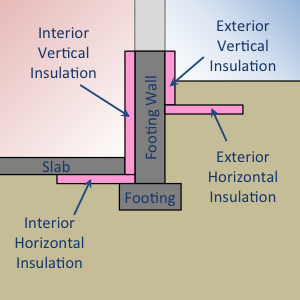
\includegraphics{media/kiva-2d-elements.png}
\caption{Structural and insulation components of Foundation:Kiva
objects\label{fig:el}}
\end{figure}

Foundation:Kiva objects define only the aspects of the foundation that
are not already defined by the one-dimensional constructions of the
respective surfaces. That is, the footing wall and slab constructions
and their relative dimensions are inferred from the respective Surface
objects (see Figure \ref{fig:surf}).

\begin{figure}
\centering
\includegraphics{media/kiva-2d-surfaces.png}
\caption{Two-dimensional interpretation of foundation surface
data\label{fig:surf}}
\end{figure}

The depth of the foundation is defined by the height of the wall surfaces
that reference the Foundation:Kiva boundary condition object. For
slab-on-grade foundations, a depth of zero is implied by having no
associated wall surfaces. Figure \ref{fig:ws} shows a slab-on-grade
foundation with whole slab insulation. Notice there are no walls
referencing the ``Foundation'' Outside Boundary Condition. In this case,
the under-slab insulation is modeled as part of the slab construction,
while the edge/gap insulation is modeled using the interior vertical
insulation fields of a Foundation:Kiva object. Note: Since there are no
wall surfaces for slab foundations, the footing wall construction is
defined within the Foundation:Kiva object (or defaulted to a 0.3m wide
cast concrete wall).

\begin{figure}
\centering
\includegraphics{media/kiva-2d-whole-slab.png}
\caption{Two-dimensional interpretation of foundation surface
data\label{fig:ws}}
\end{figure}

A walkout basement (with a variable grade along the sides; see Figure
\ref{fig:wo-r}) is best modeled using discrete quadrilateral surfaces of
stepped height for the walls as shown in Figure \ref{fig:wo-s}.

\begin{figure}
\centering
\includegraphics{media/kiva-walkout-real.png}
\caption{Example walkout basement\label{fig:wo-r}}
\end{figure}

\begin{figure}
\centering
\includegraphics{media/kiva-walkout-segs.png}
\caption{Walkout basement wall and floor surfaces (in gray) all
reference the same Foundation:Kiva object\label{fig:wo-s}}
\end{figure}

The width of the floor surface in the two-dimensional context is defined
by the area and the exposed perimeter (see
\hyperref[surfaceproperty-exposedfoundationperimeter]{SurfaceProperty:ExposedFoundationPerimeter}) of the floor surface object.
Details on this calculation can be found in the Engineering Reference
document.

Other components of the two-dimensional context are defined by the
\hyperref[foundation-kiva-settings]{Foundation:Kiva:Settings} object and applied uniformly for all instances
of Foundation:Kiva objects. These components include:

\begin{itemize}
\tightlist
\item
  Far-Field width
\item
  Deep Ground depth (and boundary type)
\item
  Soil and ground surface thermal properties
\end{itemize}

\subsubsection{Example IDF}\label{example-idf}

\begin{lstlisting}
BuildingSurface:Detailed,
  Slab Floor,         !- Name
  Floor,              !- Surface Type
  Slab Construction,  !- Construction Name
  Living Room,        !- Zone Name
  Foundation,         !- Outside Boundary Condition
  Slab Details,       !- Outside Boundary Condition Object
  No,                 !- Sun Exposure
  No,                 !- Wind Exposure
  0.0,                !- View Factor to Ground
  4,                  !- Number of Vertices
  0.0, 0.0, 0.0,      !- Vertex 1
  0.0, 20.0, 0.0,     !- Vertex 2
  20.0, 20.0, 0.0,    !- Vertex 3
  20.0, 0.0, 0.0;     !- Vertex 4

Foundation:Kiva,
  Slab Details,              !- Name
  ,                          !- Initial Indoor Air Temperature
  XPS,                       !- Interior Horizontal Insulation Material Name
  0.2,                       !- Interior Horizontal Insulation Depth
  0.6,                       !- Interior Horizontal Insulation Width
  XPS,                       !- Interior Vertical Insulation Material Name
  0.2,                       !- Interior Vertical Insulation Depth
  ,                          !- Exterior Horizontal Insulation Material Name
  ,                          !- Exterior Horizontal Insulation Depth
  ,                          !- Exterior Horizontal Insulation Width
  ,                          !- Exterior Vertical Insulation Material Name
  ,                          !- Exterior Vertical Insulation Depth
  0.2,                       !- Wall Height Above Grade
  0.3,                       !- Wall Depth Below Slab
  Slab Footing Construction; !- Footing Wall Construction Name

Material,
  XPS,    !- Name
  Rough,  !- Roughness
  0.05,   !- Thickness
  0.029,  !- Conductivity
  28,     !- Density
  1450,   !- Specific Heat
  0.9,    !- Thermal Absorptance
  0.7,    !- Solar Absorptance
  0.7;    !- Visible Absorptance

Material,
  Concrete,  !- Name
  Rough,     !- Roughness
  0.3,       !- Thickness
  1.95,      !- Conductivity
  2400,      !- Density
  900,       !- Specific Heat
  0.9,       !- Thermal Absorptance
  0.7,       !- Solar Absorptance
  0.7;       !- Visible Absorptance

Construction,
  Slab Footing Construction, !- Name
  Concrete;                  !- Outside Layer Name
\end{lstlisting}

\subsubsection{Inputs}

\paragraph{Field: Name}

The unique identifier of the Foundation:Kiva object. Referenced by a the
``Outside Boundary Condition Object'' field in a surface object.

\paragraph{Field: Initial Indoor Air Temperature}

Indoor air temperature used for Kiva initialization (prior to warmup period).
If left blank, indoor air temperature during initialization will be estimated based on zone setpoints.

\paragraph{Field: Interior Horizontal Insulation Material
Name}

A reference to a material object associated with the interior horizontal
insulation. If left blank, no interior horizontal insulation will be
used. Default: blank.

The following two fields define the placement of this material within
Kiva's two-dimensional context and are illustrated in Figure
\ref{fig:ihi}.

\begin{figure}
\centering
\includegraphics{media/kiva-2d-ihi.png}
\caption{Placement of interior horizontal insulation\label{fig:ihi}}
\end{figure}

\paragraph{Field: Interior Horizontal Insulation
Depth}

Distance from the wall top to the top of interior horizontal insulation,
in m. Required if Interior Horizontal Insulation Material Name is
defined.

\paragraph{Field: Interior Horizontal Insulation
Width}

Extent of insulation as measured from the wall interior to the edge of
interior horizontal insulation, in m. Required if Interior Horizontal
Insulation Material Name is defined.

\paragraph{Field: Interior Vertical Insulation Material
Name}

A reference to a material object associated with the interior vertical
insulation. If left blank, no interior vertical insulation will be used.
Default: blank.

The following field defines the placement of this material within Kiva's
two-dimensional context and are illustrated in Figure \ref{fig:ivi}.

\begin{figure}
\centering
\includegraphics{media/kiva-2d-ivi.png}
\caption{Placement of interior vertical insulation\label{fig:ivi}}
\end{figure}

\paragraph{Field: Interior Vertical Insulation
Depth}

Extent of insulation as measured from the wall top to the bottom edge of
the interior vertical insulation, in m. Required if Interior Vertical
Insulation Material Name is defined.

\paragraph{Field: Exterior Horizontal Insulation Material
Name}

A reference to a material object associated with the exterior horizontal
insulation. If left blank, no exterior horizontal insulation will be
used. Default: blank.

The following two fields define the placement of this material within
Kiva's two-dimensional context and are illustrated in Figure
\ref{fig:ehi}.

\begin{figure}
\centering
\includegraphics{media/kiva-2d-ehi.png}
\caption{Placement of exterior horizontal insulation\label{fig:ehi}}
\end{figure}

\paragraph{Field: Exterior Horizontal Insulation
Depth}

Distance from the wall top to the top of exterior horizontal insulation,
in m. Required if Exterior Horizontal Insulation Material Name is
defined.

\paragraph{Field: Exterior Horizontal Insulation
Width}

Extent of insulation as measured from the wall exterior to the edge of
exterior horizontal insulation, in m. Required if Exterior Horizontal
Insulation Material Name is defined.

\paragraph{Field: Exterior Vertical Insulation Material
Name}

A reference to a material object associated with the exterior vertical
insulation. If left blank, no exterior vertical insulation will be used.
Default: blank

The following field defines the placement of this material within Kiva's
two-dimensional context and are illustrated in Figure \ref{fig:evi}.

\begin{figure}
\centering
\includegraphics{media/kiva-2d-evi.png}
\caption{Placement of exterior vertical insulation\label{fig:evi}}
\end{figure}

\paragraph{Field: Exterior Vertical Insulation
Depth}

Extent of insulation as measured from the wall top to the bottom edge of
the exterior vertical insulation, in m. Required if Exterior Vertical
Insulation Material Name is defined.

\paragraph{Field: Wall Height Above
Grade}

Distance from the exterior grade to the wall top, in m. Default: 0.2 m

Figures \ref{fig:2d-w} and \ref{fig:2d-w-slab} illustrate the definition of both the ``Wall
Height Above Grade'' and the following field, ``Wall Depth Below Slab''.

\begin{figure}
\centering
\includegraphics{media/kiva-2d-wall.png}
\caption{Definition of exterior grade and footing wall depth relative to
the wall surface (for a basement foundation context)\label{fig:2d-w}}
\end{figure}

\begin{figure}
\centering
\includegraphics{media/kiva-2d-wall-slab.png}
\caption{Definition of exterior grade and footing wall depth relative to
the wall surface (for a slab foundation context)\label{fig:2d-w-slab}}
\end{figure}

\paragraph{Field: Wall Depth Below
Slab}

Distance from the slab bottom to the bottom of the foundation wall, in
m. Default: 0.0 m

Extending the wall below the slab provides a coarse approximation of the
foundation footing. Alternatively, one may use the the fields ``Footing
Material Name'' and ``Footing Depth'' to explicitly model the footing.
Note, that explicit modeling of the footing requires a higher spatial
discretization and, therefore, longer computation times.

\paragraph{Field: Footing Wall Construction
Name}

Defines the construction of the foundation footing wall for slab foundations where the foundation wall is not exposed
to the zone (and has no zone surface to explicitly assign a
construction).

By default, this is the same construction as any associated below-grade
wall surfaces, or a 0.3 m wide poured concrete wall (conductivity = 1.95
W/m-K, density = 2240 kg/m3, specific heat = 900 J/kg-K).

\paragraph{Field: Footing Material
Name}

A reference to a material object associated with the foundation footing
(typically some form of concrete). The thickness of this material is
used to determine the width of the footing. If left blank, no footing
will be used. Default: blank

The following field defines the placement of this material within Kiva's
two-dimensional context and are illustrated in Figure \ref{fig:foot}.

\begin{figure}
\centering
\includegraphics{media/kiva-2d-footing.png}
\caption{Placement of footing\label{fig:foot}}
\end{figure}

\paragraph{Field: Footing Depth}

Top-to-bottom dimension of the footing (not to be confused with its
depth in the ground). The width of the footing is defined by the
material's thickness. Default: 0.3 m.

\paragraph{Field: Custom Block \textless{}x\textgreater{} Material
Name}

A reference to a material object associated with a custom block in the
two-dimensional foundation context. The thickness of this material
determines the width of the block.

Custom blocks can be used to represent solid materials in the
two-dimensional context that are not otherwise covered by the fields
above. Examples of this might include interior finishings and insulation
(Figure \ref{fig:cw}) or backfill soil with different thermal properties
(Figure \ref{fig:cf}).

\begin{figure}
\centering
\includegraphics{media/kiva-2d-custom-ex-wall.png}
\caption{Custom blocks representing interior batt insulation and dry
wall\label{fig:cw}}
\end{figure}

\begin{figure}
\centering
\includegraphics{media/kiva-2d-custom-ex-fill.png}
\caption{Custom block representing exterior backfill\label{fig:cf}}
\end{figure}

If two or more custom blocks overlap, the final properties are
determined by the higher block number (e.g., Custom Block 4 in the input
object supersedes properties defined by Custom Block 2). All custom
blocks properties are superseded by the elements shown in Figure
\ref{fig:el}.

The following fields defines the placement of this material within
Kiva's two-dimensional context and are illustrated in Figure
\ref{fig:custom}.

\begin{figure}
\centering
\includegraphics{media/kiva-2d-custom.png}
\caption{Placement of a custom block\label{fig:custom}}
\end{figure}

\paragraph{Field: Custom Block \textless{}x\textgreater{}
Depth}

Top-to-bottom dimension of the block downward. The default is the depth
from the wall top to the top of the slab to facilitate interior
constructions. Default: Slab depth

\paragraph{Field: Custom Block \textless{}x\textgreater{} X
Position}

Position outward (+) or inward (-) relative to the foundation wall.

\paragraph{Field: Custom Block \textless{}x\textgreater{} Z
Position}

Position downward (+) relative to the foundation wall top. Default: Wall
top

\subsubsection{Outputs}

Output for surfaces with a Foundation boundary condition type will
include all opaque surface output variables except:

\begin{itemize}
\tightlist
\item
  Surface Outside Face variables (since there is no ``Outside Face'')
\item
  Surface Heat Storage variables (since this definition depends on an
  ``Outside Face'')
\item
  Surface Internal Source Location Temperature (Kiva doesn't handle
  internal sources yet, but this is a possible future enhancement)
\end{itemize}

\subsection{Foundation:Kiva:Settings}\label{foundation-kiva-settings}

This object defines settings applied across all Kiva foundation
calculations. This object is not required. If it is not defined, all
defaults will be applied.

\subsubsection{Inputs}\label{foundation-kiva-settings-inputs}

\paragraph{Field: Soil Conductivity}\label{foundation-kiva-settings-soil-conductivity}

The thermal conductivity of the soil, in W/m-K. Default: 1.73 W/m-K.

\paragraph{Field: Soil Density}\label{foundation-kiva-settings-soil-density}

The bulk density of the soil, in kg/m3. Default: 1842 kg/m3.

\paragraph{Field: Soil Specific Heat}\label{foundation-kiva-settings-soil-specific-heater}

The specific heat of the soil, in J/kg-K. Default: 419 J/kg-K

\paragraph{Field: Ground Solar Absorptivity}\label{foundation-kiva-settings-ground-solar-absorptivity}

Solar absorptivity of the exterior grade surface. Default: 0.9.

\paragraph{Field: Ground Thermal Absorptivity}\label{foundation-kiva-settings-ground-thermal-absorptivity}

Long-wave absorptivity (emissivity) of the exterior grade surface.
Default: 0.9.

\paragraph{Field: Ground Surface Roughness}\label{foundation-kiva-settings-ground-thermal-roughness}

The relief roughness of the exterior ground surface in m. Default: 0.03
m.

Estimates of surface roughnesses in m are shown in Table \ref{table:kiva-example-surface-and-roughness}.

\begin{longtable}[c]{@{}ll@{}}
\caption{Example Surface and Roughness \label{table:kiva-example-surface-and-roughness}} \tabularnewline
\toprule
Example Surface & Roughness {[}m{]} \tabularnewline
\midrule
\endfirsthead

\caption[]{Example Surface and Roughness} \tabularnewline
\toprule
Example Surface & Roughness {[}m{]} \tabularnewline
\midrule
\endhead

Concrete & 0.002 \tabularnewline
Brick & 0.003 \tabularnewline
Soil & 0.005 \tabularnewline
Gravel & 0.012 \tabularnewline
Grass & 0.030 \tabularnewline
\bottomrule
\end{longtable}

\paragraph{Field: Far-Field Width}\label{foundation-kiva-settings-far-field-width}

The distance from the wall interior to the zero horizontal heat flux
(i.e., adiabatic) far-field boundary, in m. This distance represents
either the distance halfway between this foundation and a similar
foundation of a neighboring building, or a distance adequately far from
the foundation such that it is isolated from the effects of the boundary
(typically \textgreater{}= 40 m). Default: 40 m.

\paragraph{Field: Deep-Ground Boundary Condition}\label{foundation-kiva-settings-deep-ground-boundary-condition}

Defines the type of boundary condition to apply at the Deep-Ground
Depth. Options are:

\begin{itemize}
\tightlist
\item
  ZeroFlux
\item
  GroundWater
\item
  Autoselect
\end{itemize}

ZeroFlux applies a zero vertical heat flux (i.e.~adiabatic) boundary
condition. GroundWater applies a constant temperature boundary
condition, with a temperature equal to the average outdoor air dry-bulb
temperature from the environment(s). Autoselect applies either boundary
condition depending on the elevation of the building site (Williams and
Williamson, 1989):

\[d_{wt}=0.1022\cdot d_{elev}\]

If \(d_{wt} \le\) 40 m., the GroundWater boundary is applied, otherwise
a ZeroFlux boundary is applied at 40 m. If the calculated ground water depth is
shallower than any element of the foundation construction, then the GroundWater
is applied at 1 m below the lowest element.

Default: Autoselect.

\paragraph{Field: Deep-Ground Depth}\label{foundation-kiva-settings-deep-ground-depth}

The distance from the exterior grade to the deep ground boundary, in m.
This distance represents either the distance to the ground water level,
or a distance adequately far from the foundation such that it is
isolated from the effects of the boundary (typically \textgreater{}= 40
m). Default 40 m, or the distance determined by the ``Auto'' Deep-Ground
Boundary Condition.

\paragraph{Field: Minimum Cell Dimension}\label{foundation-kiva-settings-minimum-cell-dimension}

The minimum cell dimension, in m, used in the Kiva discretization.
Default: 0.02 m.

\paragraph{Field: Maximum Cell Growth Coefficient}\label{foundation-kiva-settings-maximum-cell-growth-coefficient}

The maximum ratio of growth between neighboring cells in the direction
away from the near-field area of interest. Default: 1.50.

\paragraph{Field: Simulation Timestep}\label{foundation-kiva-settings-simulation-timestep}

This field allows the user to choose whether to calculate foundation
loads on the zone timestep or at hourly intervals. Hourly intervals will
allow for less overall computation time, but with less accuracy. Choices
are ``Hourly'' and ``Timestep''. Default: Hourly

\subsection{SurfaceProperty:ExposedFoundationPerimeter}\label{surfaceproperty-exposedfoundationperimeter}

This object (currently only used in conjunction with \hyperref[foundationkiva]{Foundation:Kiva}
boundary conditions) defines the perimeter of a foundation floor that is
exposed to the exterior environment through the floor. The user may
either define the total exposed perimeter, the fraction of the total
perimeter that is exposed, or individually define which segments of the
floor surface perimeter are exposed. This object is required for any floor surface with a \hyperref[foundationkiva]{Foundation:Kiva} boundary condition.

Figure \ref{fig:ex} illustrates how the exposed perimeter is determined
from a floor plan of the foundation level.

Some buildings may have neighboring zones with different foundation
types. For example, a crawlspace next to a garage with a slab (Figure
\ref{fig:ifw}). The foundation wall in this case is NOT considered part
of either floor's exposed perimeter, and should not reference a
Foundation boundary condition. Kiva does not calculate heat flow between
two zones through ground. In this case, it is best to approximate
interior foundation wall using an Adiabatic Outside Boundary Condition.

\begin{figure}
\centering
\includegraphics{media/kiva-exposed-perim.png}
\caption{Exposed foundation perimeter\label{fig:ex}}
\end{figure}

\begin{figure}
\centering
\includegraphics{media/kiva-interior-fnd-wall.png}
\caption{Interior foundation wall\label{fig:ifw}}
\end{figure}

\subsubsection{Inputs}\label{surfaceproperty-exposedfoundationperimeter-inputs}

\paragraph{Field: Surface Name}\label{surfaceproperty-exposedfoundationperimeter-surface-name}

Name of foundation floor surface.

\paragraph{Field: Exposed Perimeter Calculation Method}\label{field-exposed-perimeter-calculation-method}

Required key/choice field that tells which method to use to calculate the exposed foundation perimeter. Choices are:

\begin{itemize}
\item TotalExposedPerimeter: Exposed perimeter is defined as an absolute distance in m. (The Total Exposed Perimeter field should be filled.)

\item ExposedPerimeterFraction: Exposed perimeter is defined as a fraction of the total floor perimeter. (The Exposed Perimeter Fraction field should be filled.)

\item BySegment: Each segment of the floor polygon (corresponding to distance between each set of vertices) is defined as exposed (``Yes'') or not exposed (``No'') in an extensible list corresponding to the number of vertices in the floor polygon. Exposed perimeter is defined as the sum of all exposed segement lengths. (The Surface Segment \textless{}x\textgreater{}
Exposed fields should be filled.)
\end{itemize}

\paragraph{Field: Total Exposed Perimeter}\label{surfaceproperty-exposedfoundationperimeter-total-exposed-perimeter}

Total perimeter that is is exposed in m.

\paragraph{Field: Exposed Perimeter Fraction}\label{surfaceproperty-exposedfoundationperimeter-exposed-perimeter-fraction}

Fraction of the total perimeter that is exposed. Default 1.0

\paragraph{Field: Surface Segment \textless{}x\textgreater{} Exposed}\label{surfaceproperty-exposedfoundationperimeter-surface-segment-x-exposed}

Surface Segment \textless{}x\textgreater{} is the perimeter between the
\textless{}x\textgreater{}th and (\textless{}x\textgreater{}+1)th
vertices.

\subsection{SurfaceConvectionAlgorithm:Inside:AdaptiveModelSelections}\label{surfaceconvectionalgorithminsideadaptivemodelselections}

This object provides options to change the individual convection model equations for dynamic selection when using AdaptiveConvectionAlgorithm. This object is only needed to make changes to the default model selections for any or all of the surface categories. This object is for the inside face, the side of the surface facing a thermal zone.

\subsubsection{Inputs}\label{inputs-6}

\paragraph{Field: Name}\label{field-name-5}

A unique name for the object.

\paragraph{Field: Simple Buoyancy Vertical Wall Equation Source}\label{field-simple-buoyancy-vertical-wall-equation-source}

Applies to zone with no HVAC or when HVAC is off. This is for vertical walls. The key choice options include: FohannoPolidoriVerticalWall, ASHRAEVerticalWall, AlamdariHammondVerticalWall, KhalifaEq3WallAwayFromHeat, KhalifaEq6NonHeatedWalls FohannoPolidoriVerticalWall, ISO15099Windows, or UserCurve

\paragraph{Field: Simple Buoyancy Vertical Wall User Curve Name}\label{field-simple-buoyancy-vertical-wall-user-curve-name}

The SurfaceConvectionAlgorithm:UserCurve named in this field is used when the previous field is set to UserCurve

\paragraph{Field: Simple Buoyancy Stable Horizontal Equation Source}\label{field-simple-buoyancy-stable-horizontal-equation-source}

Applies to zone with no HVAC or when HVAC is off. This is for horizontal surfaces with heat flow directed for stable thermal stratification. The key choice options include: WaltonStableHorizontalOrTilt, AlamdariHammondStableHorizontal, or UserCurve

\paragraph{Field: Simple Buoyancy Stable Horizontal Equation User Curve Name}\label{field-simple-buoyancy-stable-horizontal-equation-user-curve-name}

The SurfaceConvectionAlgorithm:UserCurve named in this field is used when the previous field is set to UserCurve

\paragraph{Field: Simple Buoyancy Unstable Horizontal Equation Source}\label{field-simple-buoyancy-unstable-horizontal-equation-source}

Applies to zone with no HVAC or when HVAC is off. This is for passive horizontal surfaces with heat flow for unstable thermal stratification. The key choice options include: WaltonUnstableHorizontalOrTilt, AlamdariHammondUnstableHorizontal, or UserCurve.

\paragraph{Field: Simple Buoyancy Unstable Horizontal Equation User Curve Name}\label{field-simple-buoyancy-unstable-horizontal-equation-user-curve-name}

The SurfaceConvectionAlgorithm:UserCurve named in this field is used when the previous field is set to UserCurve.

\paragraph{Field: Simple Buoyancy Stable Tilted Equation Source}\label{field-simple-buoyancy-stable-tilted-equation-source}

Applies to zone with no HVAC or when HVAC is off. This is for tilted surfaces with heat flow for stable thermal stratification. The key choice options include: WaltonStableHorizontalOrTilt, AlamdariHammondStableHorizontal, or UserCurve

\paragraph{Field: Simple Buoyancy Stable Tilted Equation User Curve Name}\label{field-simple-buoyancy-stable-tilted-equation-user-curve-name}

The SurfaceConvectionAlgorithm:UserCurve named in this field is used when the previous field is set to UserCurve.

\paragraph{Field: Simple Buoyancy Unstable Tilted Equation Source}\label{field-simple-buoyancy-unstable-tilted-equation-source}

Applies to zone with no HVAC or when HVAC is off. This is for tilted surfaces with heat flow for unstable thermal stratification. The key choices include: WaltonUnstableHorizontalOrTilt, AlamdariHammondUnstableHorizontal, or UserCurve.

\paragraph{Field: Simple Buoyancy Unstable Tilted Equation User Curve Name}\label{field-simple-buoyancy-unstable-tilted-equation-user-curve-name}

The SurfaceConvectionAlgorithm:UserCurve named in this field is used when the previous field is set to UserCurve.

\paragraph{Field: Simple Buoyancy Windows Equation Source}\label{field-simple-buoyancy-windows-equation-source}

Applies to zone with no HVAC or when HVAC is off. This is for all window surfaces. The key choice options include: ASHRAEVerticalWall, AlamdariHammondVerticalWall, FohannoPolidoriVerticalWall, KaradagChilledCeiling, ISO15099Windows, or UserCurve.

\paragraph{Field: Simple Buoyancy Windows Equation User Curve Name}\label{field-simple-buoyancy-windows-equation-user-curve-name}

The SurfaceConvectionAlgorithm:UserCurve named in this field is used when the previous field is set to UserCurve.

\paragraph{Field: Floor Heat Ceiling Cool Vertical Wall Equation Source}\label{field-floor-heat-ceiling-cool-vertical-wall-equation-source}

Applies to zone with in-floor heating and/or in-ceiling cooling. This is for vertical walls. The key choice options include: ASHRAEVerticalWall, AlamdariHammondVerticalWall, KhalifaEq3WallAwayFromHeat, FohannoPolidoriVerticalWall, ISO15099Windows, or UserCurve.

\paragraph{Field: Floor Heat Ceiling Cool Vertical Wall Equation User Curve Name}\label{field-floor-heat-ceiling-cool-vertical-wall-equation-user-curve-name}

The SurfaceConvectionAlgorithm:UserCurve named in this field is used when the previous field is set to UserCurve.

\paragraph{Field: Floor Heat Ceiling Cool Stable Horizontal Equation Source}\label{field-floor-heat-ceiling-cool-stable-horizontal-equation-source}

Applies to zone with in-floor heating and/or in-ceiling cooling. This is for passive horizontal surfaces with heat flow for stable thermal stratification. The key choice options include: WaltonStableHorizontalOrTilt, AlamdariHammondStableHorizontal, or UserCurve.

\paragraph{Field: Floor Heat Ceiling Cool Stable Horizontal Equation User Curve Name}\label{field-floor-heat-ceiling-cool-stable-horizontal-equation-user-curve-name}

The SurfaceConvectionAlgorithm:UserCurve named in this field is used when the previous field is set to UserCurve.

\paragraph{Field: Floor Heat Ceiling Cool Unstable Horizontal Equation Source}\label{field-floor-heat-ceiling-cool-unstable-horizontal-equation-source}

Applies to zone with in-floor heating and/or in-ceiling cooling. This is for passive horizontal surfaces with heat flow for unstable thermal stratification. The key choice options include: WaltonUnstableHorizontalOrTilt, AlamdariHammondUnstableHorizontal, KhalifaEq4CeilingAwayFromHeat, or UserCurve.

\paragraph{Field: Floor Heat Ceiling Cool Unstable Horizontal Equation User Curve Name}\label{field-floor-heat-ceiling-cool-unstable-horizontal-equation-user-curve-name}

The SurfaceConvectionAlgorithm:UserCurve named in this field is used when the previous field is set to UserCurve.

\paragraph{Field: Floor Heat Ceiling Cool Heated Floor Equation Source}\label{field-floor-heat-ceiling-cool-heated-floor-equation-source}

Applies to zone with in-floor heating and/or in-ceiling cooling. This is for a floor with active heating elements. The key choice options include: WaltonUnstableHorizontalOrTilt, AlamdariHammondUnstableHorizontal, AwbiHattonHeatedFloor, or UserCurve

\paragraph{Field: Floor Heat Ceiling Cool Heated Floor Equation User Curve Name}\label{field-floor-heat-ceiling-cool-heated-floor-equation-user-curve-name}

The SurfaceConvectionAlgorithm:UserCurve named in this field is used when the previous field is set to UserCurve.

\paragraph{Field: Floor Heat Ceiling Cool Chilled Ceiling Equation Source}\label{field-floor-heat-ceiling-cool-chilled-ceiling-equation-source}

Applies to zone with in-floor heating and/or in-ceiling cooling. This is for a ceiling with active cooling elements. The key choice options include: WaltonUnstableHorizontalOrTilt, AlamdariHammondUnstableHorizontal, KaradagChilledCeiling, or UserCurve.

\paragraph{Field: Floor Heat Ceiling Cool Chilled Ceiling Equation User Curve Name}\label{field-floor-heat-ceiling-cool-chilled-ceiling-equation-user-curve-name}

The SurfaceConvectionAlgorithm:UserCurve named in this field is used when the previous field is set to UserCurve

\paragraph{Field: Floor Heat Ceiling Cool Stable Tilted Equation Source}\label{field-floor-heat-ceiling-cool-stable-tilted-equation-source}

Applies to zone with in-floor heating and/or in-ceiling cooling. This is for tilted surfaces with heat flow for stable thermal stratification. The key choice options include: WaltonStableHorizontalOrTilt, AlamdariHammondStableHorizontal, ISO15099Windows, or UserCurve.

\paragraph{Field: Floor Heat Ceiling Cool Stable Tilted Equation User Curve Name}\label{field-floor-heat-ceiling-cool-stable-tilted-equation-user-curve-name}

The SurfaceConvectionAlgorithm:UserCurve named in this field is used when the previous field is set to UserCurve.

\paragraph{Field: Floor Heat Ceiling Cool Unstable Tilted Equation Source}\label{field-floor-heat-ceiling-cool-unstable-tilted-equation-source}

Applies to zone with in-floor heating and/or in-ceiling cooling. This is for tilted surfaces with heat flow for unstable thermal stratification. The key choice options include: WaltonUnstableHorizontalOrTilt, AlamdariHammondUnstableHorizontal, ISO15099Windows, or UserCurve.

\paragraph{Field: Floor Heat Ceiling Cool Unstable Tilted Equation User Curve Name}\label{field-floor-heat-ceiling-cool-unstable-tilted-equation-user-curve-name}

The SurfaceConvectionAlgorithm:UserCurve named in this field is used when the previous field is set to UserCurve.

\paragraph{Field: Floor Heat Ceiling Cool Window Equation Source}\label{field-floor-heat-ceiling-cool-window-equation-source}

Applies to zone with in-floor heating and/or in-ceiling cooling. This is for all window surfaces. The key choice options include: ASHRAEVerticalWall, AlamdariHammondVerticalWall, ISO15099Windows, or UserCurve.

\paragraph{Field: Floor Heat Ceiling Cool Window Equation User Curve Name}\label{field-floor-heat-ceiling-cool-window-equation-user-curve-name}

The SurfaceConvectionAlgorithm:UserCurve named in this field is used when the previous field is set to UserCurve.

\paragraph{Field: Wall Panel Heating Vertical Wall Equation Source}\label{field-wall-panel-heating-vertical-wall-equation-source}

Applies to zone with in-wall panel heating. This is for vertical walls that are not actively heated. The key choice options include: ASHRAEVerticalWall, AlamdariHammondVerticalWall, KhalifaEq6NonHeatedWalls, FohannoPolidoriVerticalWall, AlamdariHammondVerticalWall, ISO15099Windows, or UserCurve.

\paragraph{Field: Wall Panel Heating Vertical Wall Equation User Curve Name}\label{field-wall-panel-heating-vertical-wall-equation-user-curve-name}

The SurfaceConvectionAlgorithm:UserCurve named in this field is used when the previous field is set to UserCurve.

\paragraph{Field: Wall Panel Heating Heated Wall Equation Source}\label{field-wall-panel-heating-heated-wall-equation-source}

Applies to zone with in-wall panel heating. This is for vertical walls that are being actively heated. The key choice options include: ASHRAEVerticalWall, AlamdariHammondVerticalWall, KhalifaEq5WallNearHeat, AwbiHattonHeatedWall, FohannoPolidoriVerticalWall, AlamdariHammondVerticalWall, or UserCurve.

\paragraph{Field: Wall Panel Heating Heated Wall Equation User Curve Name}\label{field-wall-panel-heating-heated-wall-equation-user-curve-name}

The SurfaceConvectionAlgorithm:UserCurve named in this field is used when the previous field is set to UserCurve.

\paragraph{Field: Wall Panel Heating Stable Horizontal Equation Source}\label{field-wall-panel-heating-stable-horizontal-equation-source}

Applies to zone with in-wall panel heating. This is for horizontal surfaces with heat flow directed for stable thermal stratification. The key choice options include: WaltonStableHorizontalOrTilt, AlamdariHammondStableHorizontal, or UserCurve.

\paragraph{Field: Wall Panel Heating Stable Horizontal Equation User Curve Name}\label{field-wall-panel-heating-stable-horizontal-equation-user-curve-name}

The SurfaceConvectionAlgorithm:UserCurve named in this field is used when the previous field is set to UserCurve.

\paragraph{Field: Wall Panel Heating Unstable Horizontal Equation Source}\label{field-wall-panel-heating-unstable-horizontal-equation-source}

Applies to zone with in-wall panel heating. This is for horizontal surfaces with heat flow directed for unstable thermal stratification. The key choice options include: ASHRAEVerticalWall, WaltonUnstableHorizontalOrTilt, AlamdariHammondUnstableHorizontal, KhalifaEq7Ceiling, or UserCurve

\paragraph{Field: Wall Panel Heating Unstable Horizontal Equation User Curve Name}\label{field-wall-panel-heating-unstable-horizontal-equation-user-curve-name}

The SurfaceConvectionAlgorithm:UserCurve named in this field is used when the previous field is set to UserCurve.

\paragraph{Field: Wall Panel Heating Stable Tilted Equation Source}\label{field-wall-panel-heating-stable-tilted-equation-source}

Applies to zone with in-wall panel heating. This is for tilted surfaces with heat flow for stable thermal stratification. The key choice options include: WaltonStableHorizontalOrTilt, AlamdariHammondStableHorizontal, ISO15099Windows, or UserCurve.

\paragraph{Field: Wall Panel Heating Stable Tilted Equation User Curve Name}\label{field-wall-panel-heating-stable-tilted-equation-user-curve-name}

The SurfaceConvectionAlgorithm:UserCurve named in this field is used when the previous field is set to UserCurve

\paragraph{Field: Wall Panel Heating Unstable Tilted Equation Source}\label{field-wall-panel-heating-unstable-tilted-equation-source}

Applies to zone with in-wall panel heating. This is for tilted surfaces with heat flow for unstable thermal stratification. The key choice options include: WaltonUnstableHorizontalOrTilt, AlamdariHammondUnstableHorizontal, ISO15099Windows, or UserCurve.

\paragraph{Field: Wall Panel Heating Unstable Tilted Equation User Curve Name}\label{field-wall-panel-heating-unstable-tilted-equation-user-curve-name}

The SurfaceConvectionAlgorithm:UserCurve named in this field is used when the previous field is set to UserCurve.

\paragraph{Field: Wall Panel Heating Window Equation Source}\label{field-wall-panel-heating-window-equation-source}

Applies to zone with in-wall panel heating. This is for all window surfaces. The key choice options include: ASHRAEVerticalWall, AlamdariHammondVerticalWall, FohannoPolidoriVerticalWall, ISO15099Windows, or UserCurve.

\paragraph{Field: Wall Panel Heating Window Equation User Curve Name}\label{field-wall-panel-heating-window-equation-user-curve-name}

The SurfaceConvectionAlgorithm:UserCurve named in this field is used when the previous field is set to UserCurve.

\paragraph{Field: Convective Zone Heater Vertical Wall Equation Source}\label{field-convective-zone-heater-vertical-wall-equation-source}

Applies to zone with convective heater. This is for vertical walls not directly affected by heater. The key choice options include: ASHRAEVerticalWall, AlamdariHammondVerticalWall, KhalifaEq3WallAwayFromHeat, KhalifaEq6NonHeatedWalls, FohannoPolidoriVerticalWall, ISO15099Windows, or UserCurve

\paragraph{Field: Convective Zone Heater Vertical Wall Equation User Curve Name}\label{field-convective-zone-heater-vertical-wall-equation-user-curve-name}

The SurfaceConvectionAlgorithm:UserCurve named in this field is used when the previous field is set to UserCurve.

\paragraph{Field: Convective Zone Heater Vertical Walls Near Heater Equation Source}\label{field-convective-zone-heater-vertical-walls-near-heater-equation-source}

Applies to zone with convective heater. This is for vertical walls that are directly affected by heater. Walls are considered ``near'' when listed in field set for Fraction of Radiant Energy to Surface. The key choice options include: ASHRAEVerticalWall, AlamdariHammondVerticalWall, KhalifaEq5WallNearHeat, AwbiHattonHeatedWall, FohannoPolidoriVerticalWall, ISO15099Windows, or UserCurve.

\paragraph{Field: Convective Zone Heater Vertical Walls Near Heater Equation User Curve Name}\label{field-convective-zone-heater-vertical-walls-near-heater-equation-user-curve-name}

The SurfaceConvectionAlgorithm:UserCurve named in this field is used when the previous field is set to UserCurve.

\paragraph{Field: Convective Zone Heater Stable Horizontal Equation Source}\label{field-convective-zone-heater-stable-horizontal-equation-source}

Applies to zone with convective heater. This is for horizontal surfaces with heat flow directed for stable thermal stratification. The key choice options include: WaltonStableHorizontalOrTilt, AlamdariHammondStableHorizontal, or UserCurve.

\paragraph{Field: Convective Zone Heater Stable Horizontal Equation User Curve Name}\label{field-convective-zone-heater-stable-horizontal-equation-user-curve-name}

The SurfaceConvectionAlgorithm:UserCurve named in this field is used when the previous field is set to UserCurve

\paragraph{Field: Convective Zone Heater Unstable Horizontal Equation Source}\label{field-convective-zone-heater-unstable-horizontal-equation-source}

Applies to zone with convective heater. This is for horizontal surfaces with heat flow directed for unstable thermal stratification. The key choice options include: WaltonUnstableHorizontalOrTilt, AlamdariHammondUnstableHorizontal, KhalifaEq4CeilingAwayFromHeat, KhalifaEq7Ceiling, or UserCurve.

\paragraph{Field: Convective Zone Heater Unstable Horizontal Equation User Curve Name}\label{field-convective-zone-heater-unstable-horizontal-equation-user-curve-name}

The SurfaceConvectionAlgorithm:UserCurve named in this field is used when the previous field is set to UserCurve.

\paragraph{Field: Convective Zone Heater Stable Tilted Equation Source}\label{field-convective-zone-heater-stable-tilted-equation-source}

Applies to zone with convective heater. This is for tilted surfaces with heat flow for stable thermal stratification. The key choice options include: WaltonStableHorizontalOrTilt, AlamdariHammondStableHorizontal, or UserCurve.

\paragraph{Field: Convective Zone Heater Stable Tilted Equation User Curve Name}\label{field-convective-zone-heater-stable-tilted-equation-user-curve-name}

The SurfaceConvectionAlgorithm:UserCurve named in this field is used when the previous field is set to UserCurve.

\paragraph{Field: Convective Zone Heater Unstable Tilted Equation Source}\label{field-convective-zone-heater-unstable-tilted-equation-source}

Applies to zone with convective heater. This is for tilted surfaces with heat flow for unstable thermal stratification. The key choice options include: WaltonUnstableHorizontalOrTilt, AlamdariHammondUnstableHorizontal, or UserCurve.

\paragraph{Field: Convective Zone Heater Unstable Tilted Equation User Curve Name}\label{field-convective-zone-heater-unstable-tilted-equation-user-curve-name}

The SurfaceConvectionAlgorithm:UserCurve named in this field is used when the previous field is set to UserCurve.

\paragraph{Field: Convective Zone Heater Windows Equation Source}\label{field-convective-zone-heater-windows-equation-source}

Applies to zone with convective heater. This is for all window surfaces. The key choice options include: ASHRAEVerticalWall, AlamdariHammondVerticalWall, KhalifaEq3WallAwayFromHeat, FohannoPolidoriVerticalWall, ISO15099Windows, or UserCurve.

\paragraph{Field: Convective Zone Heater Windows Equation User Curve Name}\label{field-convective-zone-heater-windows-equation-user-curve-name}

The SurfaceConvectionAlgorithm:UserCurve named in this field is used when the previous field is set to UserCurve.

\paragraph{Field: Central Air Diffuser Wall Equation Source}\label{field-central-air-diffuser-wall-equation-source}

Applies to zone with mechanical forced central air with diffusers. This is for all wall surfaces. The key choice options include: ASHRAEVerticalWall, FisherPedersenCeilingDiffuserWalls, AlamdariHammondVerticalWall, BeausoleilMorrisonMixedAssistedWall, BeausoleilMorrisonMixedOpposingWall, FohannoPolidoriVerticalWall, ISO15099Windows, GoldsteinNovoselacCeilingDiffuserWalls, or UserCurve

\paragraph{Field: Central Air Diffuser Wall Equation User Curve Name}\label{field-central-air-diffuser-wall-equation-user-curve-name}

The SurfaceConvectionAlgorithm:UserCurve named in this field is used when the previous field is set to UserCurve.

\paragraph{Field: Central Air Diffuser Ceiling Equation Source}\label{field-central-air-diffuser-ceiling-equation-source}

Applies to zone with mechanical forced central air with diffusers. This is for all ceiling surfaces. The key choice options include: FisherPedersenCeilingDiffuserCeiling, BeausoleilMorrisonMixedStableCeiling, BeausoleilMorrisonMixedUnstableCeiling, or UserCurve.

\paragraph{Field: Central Air Diffuser Ceiling Equation User Curve Name}\label{field-central-air-diffuser-ceiling-equation-user-curve-name}

The SurfaceConvectionAlgorithm:UserCurve named in this field is used when the previous field is set to UserCurve.

\paragraph{Field: Central Air Diffuser Floor Equation Source}\label{field-central-air-diffuser-floor-equation-source}

Applies to zone with mechanical forced central air with diffusers. This is for all floor surfaces. The key choice options include: FisherPedersenCeilingDiffuserFloor, BeausoleilMorrisonMixedStableFloor, BeausoleilMorrisonMixedUnstableFloor, GoldsteinNovoselacCeilingDiffuserFloor, or UserCurve.

\paragraph{Field: Central Air Diffuser Floor Equation User Curve Name}\label{field-central-air-diffuser-floor-equation-user-curve-name}

The SurfaceConvectionAlgorithm:UserCurve named in this field is used when the previous field is set to UserCurve.

\paragraph{Field: Central Air Diffuser Window Equation Source}\label{field-central-air-diffuser-window-equation-source}

Applies to zone with mechanical forced central air with diffusers. This is for all window surfaces. The key choice options include: ASHRAEVerticalWall, FisherPedersenCeilingDiffuserWalls, BeausoleilMorrisonMixedAssistedWall, BeausoleilMorrisonMixedOpposingWall, FohannoPolidoriVerticalWall, AlamdariHammondVerticalWall, ISO15099Windows, GoldsteinNovoselacCeilingDiffuserWindow, or UserCurve.

\paragraph{Field: Central Air Diffuser Window Equation User Curve Name}\label{field-central-air-diffuser-window-equation-user-curve-name}

The SurfaceConvectionAlgorithm:UserCurve named in this field is used when the previous field is set to UserCurve

\paragraph{Field: Mechanical Zone Fan Circulation Vertical Wall Equation Source}\label{field-mechanical-zone-fan-circulation-vertical-wall-equation-source}

The key choice options include: KhalifaEq3WallAwayFromHeat, ASHRAEVerticalWall, FisherPedersenCeilingDiffuserWalls, AlamdariHammondVerticalWall, BeausoleilMorrisonMixedAssistedWall, BeausoleilMorrisonMixedOpposingWall, FohannoPolidoriVerticalWall, ISO15099Windows, GoldsteinNovoselacCeilingDiffuserWalls, or UserCurve.

\paragraph{Field: Mechanical Zone Fan Circulation Vertical Wall Equation User Curve Name}\label{field-mechanical-zone-fan-circulation-vertical-wall-equation-user-curve-name}

The SurfaceConvectionAlgorithm:UserCurve named in this field is used when the previous field is set to UserCurve

\paragraph{Field: Mechanical Zone Fan Circulation Stable Horizontal Equation Source}\label{field-mechanical-zone-fan-circulation-stable-horizontal-equation-source}

The key choice options include: WaltonStableHorizontalOrTilt, AlamdariHammondStableHorizontal, or UserCurve.

\paragraph{Field: Mechanical Zone Fan Circulation Stable Horizontal Equation User Curve Name}\label{field-mechanical-zone-fan-circulation-stable-horizontal-equation-user-curve-name}

The SurfaceConvectionAlgorithm:UserCurve named in this field is used when the previous field is set to UserCurve.

\paragraph{Field: Mechanical Zone Fan Circulation Unstable Horizontal Equation Source}\label{field-mechanical-zone-fan-circulation-unstable-horizontal-equation-source}

The key choice options include: KhalifaEq4CeilingAwayFromHeat, WaltonUnstableHorizontalOrTilt, AlamdariHammondUnstableHorizontal, or UserCurve.

\paragraph{Field: Mechanical Zone Fan Circulation Unstable Horizontal Equation User Curve Name}\label{field-mechanical-zone-fan-circulation-unstable-horizontal-equation-user-curve-name}

The SurfaceConvectionAlgorithm:UserCurve named in this field is used when the previous field is set to UserCurve.

\paragraph{Field: Mechanical Zone Fan Circulation Stable Tilted Equation Source}\label{field-mechanical-zone-fan-circulation-stable-tilted-equation-source}

The key choice options include: WaltonStableHorizontalOrTilt or UserCurve

\paragraph{Field Mechanical Zone Fan Circulation Stable Tilted Equation User Curve Name}\label{field-mechanical-zone-fan-circulation-stable-tilted-equation-user-curve-name}

The SurfaceConvectionAlgorithm:UserCurve named in this field is used when the previous field is set to UserCurve.

\paragraph{Field: Mechanical Zone Fan Circulation Unstable Tilted Equation Source}\label{field-mechanical-zone-fan-circulation-unstable-tilted-equation-source}

The key choice options include: WaltonUnstableHorizontalOrTilt, AlamdariHammondUnstableHorizontal, or UserCurve.

\paragraph{Field: Mechanical Zone Fan Circulation Unstable Tilted Equation User Curve Name}\label{field-mechanical-zone-fan-circulation-unstable-tilted-equation-user-curve-name}

The SurfaceConvectionAlgorithm:UserCurve named in this field is used when the previous field is set to UserCurve.

\paragraph{Field: Mechanical Zone Fan Circulation Window Equation Source}\label{field-mechanical-zone-fan-circulation-window-equation-source}

The key choice options include: ASHRAEVerticalWall, AlamdariHammondVerticalWall, FohannoPolidoriVerticalWall, ISO15099Windows, GoldsteinNovoselacCeilingDiffuserWindow, or UserCurve.

\paragraph{Field: Mechanical Zone Fan Circulation Unstable Tilted Equation User Curve Name}\label{field-mechanical-zone-fan-circulation-unstable-tilted-equation-user-curve-name-1}

The SurfaceConvectionAlgorithm:UserCurve named in this field is used when the previous field is set to UserCurve

\paragraph{Field: Mixed Regime Buoyancy Assisting Flow on Walls Equation Source}\label{field-mixed-regime-buoyancy-assisting-flow-on-walls-equation-source}

The key choice options include: BeausoleilMorrisonMixedAssistedWall, AlamdariHammondVerticalWall, FohannoPolidoriVerticalWall, ASHRAEVerticalWall, FisherPedersenCeilingDiffuserWalls, GoldsteinNovoselacCeilingDiffuserWalls, or UserCurve.

\paragraph{Field: Mixed Regime Buoyancy Assisting Flow on Walls Equation User Curve Name}\label{field-mixed-regime-buoyancy-assisting-flow-on-walls-equation-user-curve-name}

The SurfaceConvectionAlgorithm:UserCurve named in this field is used when the previous field is set to UserCurve.

\paragraph{Field: Mixed Regime Buoyancy Opposing Flow on Walls Equation Source}\label{field-mixed-regime-buoyancy-oppossing-flow-on-walls-equation-source}

The key choice options include: BeausoleilMorrisonMixedOpposingWall, AlamdariHammondVerticalWall, FohannoPolidoriVerticalWall, ASHRAEVerticalWall, FisherPedersenCeilingDiffuserWalls, GoldsteinNovoselacCeilingDiffuserWalls, or UserCurve

\paragraph{Field: Mixed Regime Buoyancy Opposing Flow on Walls Equation User Curve Name}\label{field-mixed-regime-buoyancy-oppossing-flow-on-walls-equation-user-curve-name}

The SurfaceConvectionAlgorithm:UserCurve named in this field is used when the previous field is set to UserCurve

\paragraph{Field: Mixed Regime Stable Floor Equation Source}\label{field-mixed-regime-stable-floor-equation-source}

The key choice options include: BeausoleilMorrisonMixedStableFloor, WaltonStableHorizontalOrTilt, AlamdariHammondStableHorizontal, or UserCurve

\paragraph{Field: Mixed Regime Stable Floor Equation User Curve Name}\label{field-mixed-regime-stable-floor-equation-user-curve-name}

The SurfaceConvectionAlgorithm:UserCurve named in this field is used when the previous field is set to UserCurve.

\paragraph{Field: Mixed Regime Unstable Floor Equation Source}\label{field-mixed-regime-unstable-floor-equation-source}

The key choice options include: BeausoleilMorrisonMixedUnstableFloor, WaltonUnstableHorizontalOrTilt, AlamdariHammondUnstableHorizontal, or UserCurve.

\paragraph{Field: Mixed Regime Unstable Floor Equation User Curve Name}\label{field-mixed-regime-unstable-floor-equation-user-curve-name}

The SurfaceConvectionAlgorithm:UserCurve named in this field is used when the previous field is set to UserCurve.

\paragraph{Field: Mixed Regime Stable Ceiling Equation Source}\label{field-mixed-regime-stable-ceiling-equation-source}

The key choice options include: BeausoleilMorrisonMixedStableCeiling, WaltonStableHorizontalOrTilt, AlamdariHammondStableHorizontal, or UserCurve.

\paragraph{Field: Mixed Regime Stable Ceiling Equation User Curve Name}\label{field-mixed-regime-stable-ceiling-equation-user-curve-name}

The SurfaceConvectionAlgorithm:UserCurve named in this field is used when the previous field is set to UserCurve.

\paragraph{Field: Mixed Regime Unstable Ceiling Equation Source}\label{field-mixed-regime-unstable-ceiling-equation-source}

The key choice options include: BeausoleilMorrisonMixedUnstableCeiling, WaltonUnstableHorizontalOrTilt, AlamdariHammondUnstableHorizontal, or UserCurve.

\paragraph{Field: Mixed Regime Unstable Ceiling Equation User Curve Name}\label{field-mixed-regime-unstable-ceiling-equation-user-curve-name}

The SurfaceConvectionAlgorithm:UserCurve named in this field is used when the previous field is set to UserCurve.

\paragraph{Field: Mixed Regime Window Equation Source}\label{field-mixed-regime-window-equation-source}

The key choice options include: GoldsteinNovoselacCeilingDiffuserWindow, ISO15099Windows, or UserCurve.

\paragraph{Field: Mixed Regime Window Equation User Curve Name}\label{field-mixed-regime-window-equation-user-curve-name}

The SurfaceConvectionAlgorithm:UserCurve named in this field is used when the previous field is set to UserCurve.

\subsection{SurfaceConvectionAlgorithm:Outside:AdaptiveModelSelections}\label{surfaceconvectionalgorithmoutsideadaptivemodelselections}

Options to change the individual convection model equations for dynamic selection when using AdaptiveConvectionAlgorithm. This object is only needed to make changes to the default model selections for any or all of the surface categories. This object is for the outside face, the side of the surface facing away from the thermal zone.

\subsubsection{Inputs}\label{inputs-7}

\paragraph{Field: Name}\label{field-name-6}

A unique name for the object

\paragraph{Field: Wind Convection Windward Vertical Wall Equation Source}\label{field-wind-convection-windward-vertical-wall-equation-source}

This is for just the wind-driven component of the total convection coefficient. The key choice options include: SimpleCombined, TARPWindward, MoWiTTWindward, DOE2Windward, NusseltJurges, McAdams, Mitchell, Blocken, Emmel, or UserCurve.

\paragraph{Field: Wind Convection Windward Equation Vertical Wall User Curve Name}\label{field-wind-convection-windward-equation-vertical-wall-user-curve-name}

The SurfaceConvectionAlgorithm:UserCurve named in this field is used when the previous field is set to UserCurve.

\paragraph{Field: Wind Convection Leeward Vertical Wall Equation Source}\label{field-wind-convection-leeward-vertical-wall-equation-source}

This is for just the wind-driven component of the total convection coefficient. The key choice options include: SimpleCombined, TARPLeeward, MoWiTTLeeward, DOE2Leeward, Emmel, NusseltJurges, McAdams, Mitchell, or UserCurve.

\paragraph{Field: Wind Convection Leeward Vertical Wall Equation User Curve Name}\label{field-wind-convection-leeward-vertical-wall-equation-user-curve-name}

The SurfaceConvectionAlgorithm:UserCurve named in this field is used when the previous field is set to UserCurve.

\paragraph{Field: Wind Convection Horizontal Roof Equation Source}\label{field-wind-convection-horizontal-roof-equation-source}

This is for just the wind-driven component of the total convection coefficient. The key choice options include: SimpleCombined, TARPWindward, MoWiTTWindward, DOE2Windward, NusseltJurges, McAdams, Mitchell, Blocken, Emmel, ClearRoof, or UserCurve.

\paragraph{Field: Wind Convection Horizontal Roof User Curve Name}\label{field-wind-convection-horizontal-roof-user-curve-name}

The SurfaceConvectionAlgorithm:UserCurve named in this field is used when the previous field is set to UserCurve.

\paragraph{Field: Natural Convection Vertical Wall Equation Source}\label{field-natural-convection-vertical-wall-equation-source}

This is for just the natural convection portion of the total film coefficient. This is for vertical walls. The key choice options include: ASHRAEVerticalWall, AlamdariHammondVerticalWall, FohannoPolidoriVerticalWall, ISO15099Windows, UserCurve, or None.

\paragraph{Field: Natural Convection Vertical Wall Equation User Curve Name}\label{field-natural-convection-vertical-wall-equation-user-curve-name}

The SurfaceConvectionAlgorithm:UserCurve named in this field is used when the previous field is set to UserCurve.

\paragraph{Field: Natural Convection Stable Horizontal Equation Source}\label{field-natural-convection-stable-horizontal-equation-source}

This is for just the natural convection portion of the total film coefficient. This is for horizontal surfaces with heat flow directed for stable thermal stratification. The key choice options include: WaltonStableHorizontalOrTilt, AlamdariHammondStableHorizontal, UserCurve, or None.

\paragraph{Field: Natural Convection Stable Horizontal Equation User Curve Name}\label{field-natural-convection-stable-horizontal-equation-user-curve-name}

The SurfaceConvectionAlgorithm:UserCurve named in this field is used when the previous field is set to UserCurve.

\paragraph{Field: Natural Convection Unstable Horizontal Equation Source}\label{field-natural-convection-unstable-horizontal-equation-source}

This is for just the natural convection portion of the total film coefficient. This is for horizontal surfaces with heat flow directed for unstable thermal stratification. The key choice options include: WaltonUnstableHorizontalOrTilt, AlamdariHammondUnstableHorizontal, UserCurve, or None

\paragraph{Field: Natural Convection Unstable Horizontal Equation User Curve Name}\label{field-natural-convection-unstable-horizontal-equation-user-curve-name}

The SurfaceConvectionAlgorithm:UserCurve named in this field is used when the previous field is set to UserCurve.

\subsection{SurfaceConvectionAlgorithm:Inside:UserCurve}\label{surfaceconvectionalgorithminsideusercurve}

This object is used to describe a custom model equation for surface convection heat transfer coefficients. If more than one curve is referenced, or non-blank, then they are all used and the result is the simple addition of all the curve results.

\subsubsection{Inputs}\label{inputs-8}

\paragraph{Field: Name}\label{field-name-7}

Unique name of input object.

\paragraph{Field: Reference Temperature for Convection Heat Transfer}\label{field-reference-temperature-for-convection-heat-transfer}

This field controls the nature of the reference temperature used with convection coefficient when calculating the heat flow at the surface. Select one of the three choices: MeanAirTemperature, AdjacentAirTemperature, SupplyAirTemperature. MeanAirTemperature is the typical application for the classic convection model used with the complete mixing of room air. AdjacentAirTemperature applies when used with Roomair models that account for temperature variations within the zone air and directs the model to use the temperature near the surface rather than the average for the entire zone. SupplyAirTemperature directs the model to use the supply air conditions for the heat transfer conditions.

\paragraph{Field: Hc Function of Temperature Difference Curve Name}\label{field-hc-function-of-temperature-difference-curve-name}

This field contains the name of separate performance curve or table object that describes \emph{h\(_{c}\)}, the convection coefficient, as a function of temperature difference. The curve's ``x'' is absolute value of delta-T (Surface temperature minus air temperature, (C))

\paragraph{Field: Hc Function of Temperature Difference Divided by Height Curve Name}\label{field-hc-function-of-temperature-difference-divided-by-height-curve-name}

This field contains the name of separate performance curve or table object that describes \emph{h\(_{c}\)}, the convection coefficient, as a function of temperature difference divided by height. The curve's ``x'' is absolute value of delta-T/Height (Surface temp minus Air temp)/(vertical length scale), (C/m). For an inside face, the vertical length scale is the zone's interior height.

\paragraph{Field: Hc Function of Air Change Rate Curve Name}\label{field-hc-function-of-air-change-rate-curve-name}

This field contains the name of separate performance curve or table object that describes \emph{h\(_{c}\)}, the convection coefficient, as a function of air change rate. The curve's ``x'' is mechanical ACH (Air Changes per hour from mechanical air system), (1/hr)

\paragraph{Field: Hc Function of Air System Volume Flow Rate Divided by Zone Perimeter Length Curve Name}\label{field-hc-function-of-air-system-volume-flow-rate-divided-by-zone-perimeter-length-curve-name}

This field contains the name of separate performance curve or table object that describes \emph{h\(_{c}\)}, the convection coefficient, as a function of air change rate divided perimeter scale. Curve's ``x'' is mechanical system air flow rate (m\(^{3}\)/s) divided by zone's length along exterior walls (m).

\subsection{SurfaceConvectionAlgorithm:Outside:UserCurve}\label{surfaceconvectionalgorithmoutsideusercurve}

This object is used to describe a custom model equation for surface convection heat transfer coefficients. If more than one curve is referenced, or non-blank, then they are all used and the result is the simple addition of all the curve results.

\subsubsection{Inputs}\label{inputs-9}

\paragraph{Field: Name}\label{field-name-8}

Unique name of input object.

\paragraph{Field: Wind Speed Type for Curve}\label{field-wind-speed-type-for-curve}

This field specifies what sort of wind velocity data should be used in when evaluating the curve in the following field. There are for key choice options. ``WeatherFile'' directs using the unmodified value from the epw file or design weather data. ``HeightAdjust'' uses the value from the epw file modified for height above ground, as determined by the z coordinate, using the site terrain and weather station information. ``ParallelComponent'' uses the value from the epw file modified to take just the velocity component that is parallel to the surface. ``ParallelComponentHeightAdjust'' uses the height adjusted wind velocity and then computes the parallel component.

\paragraph{Field: Hf Function of Wind Speed Curve Name}\label{field-hf-function-of-wind-speed-curve-name}

This field contains the name of separate performance curve or table object that describes \emph{h\(_{f}\)}, the forced convection coefficient, as a function of wind speed. The curve's ``x'' is wind speed as defined by the method chosen in the previous field.

\paragraph{Field: Hn Function of Temperature Difference Curve Name}\label{field-hn-function-of-temperature-difference-curve-name}

This field contains the name of separate performance curve or table object that describes \emph{h\(_{n}\)}, the natural convection coefficient, as a function of temperature difference. Curve's ``x'' is absolute value of delta-T (Surface temperature minus air temperature, (C))

\paragraph{Field: Hc Function of Temperature Difference Divided by Height Curve Name}\label{field-hc-function-of-temperature-difference-divided-by-height-curve-name-1}

This field contains the name of separate performance curve or table object that describes \emph{h\(_{n}\)}, the natural convection coefficient, as a function of temperature difference divided by height. Curve's ``x'' is absolute value of delta-T/Height (Surface temp minus Air temp)/(vertical length scale), (C/m). For an outside face the vertical length scale is the exterior facade's overall height.

\subsection{SurfaceProperty:ConvectionCoefficients}\label{surfacepropertyconvectioncoefficients}

The convection coefficients of each surface, both exterior and interior, are automatically calculated during EnergyPlus execution. These calculations are ``governed'' by other objects such as the \hyperref[surfaceconvectionalgorithminside]{SurfaceConvectionAlgorithm:Inside} (overall default), the Zone object's field called Zone Inside Convection Algorithm (Zone Default), the and the \hyperref[surfaceconvectionalgorithmoutside]{SurfaceConvectionAlgorithm:Outside} (overall default), and/or the Zone object's field called Zone Outside Convection Algorithm (Zone Default). Usually, that will be enough flexibility for most users. However, if you need to match pre-existing convection coefficients (from another program) or are trying to match a test suite of results, you may wish to use the ``override'' convection coefficients in the following object. This object allows for a single surface to be given specific convection coefficients.

Note that using these in conjunction, in particular, the ``Simple'' option on either the Outside Convection Algorithm or the Zone Outside Convection Algorithm field will result in a combined coefficient regardless of choice chosen here.

\begin{callout}
Note that surfaces with ``\hyperref[surfacepropertyothersidecoefficients]{SurfaceProperty:OtherSideCoefficients}'' cannot use this object with the ``outside'' coefficient -- attempting to do so will cause a severe error; \hyperref[surfacepropertyothersidecoefficients]{SurfaceProperty:OtherSideCoefficients} surfaces can apply an ``inside'' coefficient. And, surfaces with ``Ground'' exposure do not use the ``outside'' coefficient that might be supplied here. Note, too, that some lower boundaries are used regardless by certain surface types (i.e.~\hyperref[window]{Window}) or certain algorithm types.
\end{callout}

\subsubsection{Inputs}\label{inputs-10}

\paragraph{Field: Surface Name}\label{field-surface-name-2}

This field is the applicable surface name for the user supplied convection coefficient.

\paragraph{Fields (Convection Location, Type, Coefficient \& Schedule Name)}\label{fields-convection-location-type-coefficient-schedule-name}

For simplicity, the descriptions of these field occur together -- however, the fields are used sequentially when put into the IDF file (reference the IDF examples following the descriptions).

\paragraph{Field: Convection Coefficient 1 Location}\label{field-convection-coefficient-1-location}

\paragraph{Field: Convection Coefficient 2 Location}\label{field-convection-coefficient-2-location}

This field contains the word ``Outside'' or ``Inside'' depending on which location is being described.

\paragraph{Field: Convection Coefficient 1 Type}\label{field-convection-coefficient-1-type}

\paragraph{Field: Convection Coefficient 2 Type}\label{field-convection-coefficient-2-type}

The entries can be of several types: Value (simple numeric value), Schedule (name of schedule with the values), the usual key choices for overall models for Outside or Inside (Simple, SimpleCombined, TARP, AdaptiveConvectionAlgorithm etc.), the key choices for individual convection equations used for customizing the adaptive algorithm, or a custom user defined correlation. The field should contain one of the keys listed in the table below along with face they can be applied. The definitions of the models and key choices are discussed under \hyperref[surfaceconvectionalgorithminside]{SurfaceConvectionAlgorithm:Inside}, \hyperref[surfaceconvectionalgorithmoutside]{SurfaceConvectionAlgorithm:Outside}, \hyperref[surfaceconvectionalgorithminsideadaptivemodelselections]{SurfaceConvectionAlgorithm:Inside:AdaptiveModelSelections}, and \hyperref[surfaceconvectionalgorithmoutsideadaptivemodelselections]{SurfaceConvectionAlgorithm:Outside:AdaptiveModelSelections}.

\begin{longtable}[c]{p{3.49in}p{2.5in}}
\toprule
Key choice & Applies to Inside or Outside \tabularnewline
\midrule
\endfirsthead

\toprule
Key choice & Applies to Inside or Outside \tabularnewline
\midrule
\endhead

Value & Both \tabularnewline
Schedule & Both \tabularnewline
Simple & Inside \tabularnewline
SimpleCombined & Outside \tabularnewline
TARP & Both \tabularnewline
DOE-2 & Outside \tabularnewline
MoWitt & Outside \tabularnewline
AdaptiveConvectionAlgorithm & Both \tabularnewline
ASHRAEVerticalWall~~~ & Both \tabularnewline
WaltonUnstableHorizontalOrTilt & Both \tabularnewline
WaltonStableHorizontalOrTilt & Both \tabularnewline
FisherPedersenCeilingDiffuserWalls & Inside \tabularnewline
FisherPedersenCeilingDiffuserCeiling & Inside \tabularnewline
FisherPedersenCeilingDiffuserFloor & Inside \tabularnewline
AlamdariHammondStableHorizontal & Both \tabularnewline
AlamdariHammondUnstableHorizontal & Both \tabularnewline
AlamdariHammondVerticalWall & Both \tabularnewline
KhalifaEq3WallAwayFromHeat & Inside \tabularnewline
KhalifaEq4CeilingAwayFromHeat & Inside \tabularnewline
KhalifaEq5WallNearHeat & Inside \tabularnewline
KhalifaEq6NonHeatedWalls & Inside \tabularnewline
KhalifaEq7Ceiling & Inside \tabularnewline
AwbiHattonHeatedFloor & Inside \tabularnewline
AwbiHattonHeatedWall & Inside \tabularnewline
BeausoleilMorrisonMixedAssistedWall & Inside \tabularnewline
BeausoleilMorrisonMixedOpposingWall & Inside \tabularnewline
BeausoleilMorrisonMixedStableFloor & Inside \tabularnewline
BeausoleilMorrisonMixedUnstableFloor & Inside \tabularnewline
BeausoleilMorrisonMixedStableCeiling & Inside \tabularnewline
BeausoleilMorrisonMixedUnstableCeiling & Inside \tabularnewline
FohannoPolidoriVerticalWall~~~~~~ & Both \tabularnewline
KaradagChilledCeiling & Inside \tabularnewline
ISO15099Windows & Inside \tabularnewline
GoldsteinNovoselacCeilingDiffuserWindow & Inside \tabularnewline
GoldsteinNovoselacCeilingDiffuserWalls & Inside \tabularnewline
GoldsteinNovoselacCeilingDiffuserFloor & Inside \tabularnewline
SimpleCombined~~~~~ & Outside \tabularnewline
NusseltJurges & Outside \tabularnewline
McAdams & Outside \tabularnewline
Mitchell & Outside \tabularnewline
BlockenWindard & Outside \tabularnewline
Emmel & Outside \tabularnewline
ClearRoof & Outside \tabularnewline
UserCurve & Both \tabularnewline
\bottomrule
\end{longtable}

\paragraph{Field: Convection Coefficient 1}\label{field-convection-coefficient-1}

\paragraph{Field: Convection Coefficient 2}\label{field-convection-coefficient-2}

If the Convection type was ``Value'', then this field is filled and contains the simple value to be used. Otherwise, this can be blank.

\paragraph{Field: Convection Coefficient 1 Schedule Name}\label{field-convection-coefficient-1-schedule-name}

\paragraph{Field: Convection Coefficient 2 Schedule Name}\label{field-convection-coefficient-2-schedule-name}

If the Convection type was ``Schedule'', then this field contains the name of a schedule describing the value to be used during the time intervals for the schedule.

The complete IDD definition for the ConvectionCoefficients object follows:

\paragraph{Field: Convection Coefficient 1 User Curve Name}\label{field-convection-coefficient-1-user-curve-name}

\paragraph{Field: Convection Coefficient 2 User Curve Name}\label{field-convection-coefficient-2-user-curve-name}

If the Convection type was ``UserCurve'', then this field contains the name of a SurfaceConvectionAlgorithm:UserCurve input object describing the model equations to be used during the time intervals for the schedule.

In IDF usage:

\begin{lstlisting}

SurfaceProperty:ConvectionCoefficients,
  Zn001:Wall001,  ! Surface Name
  Outside,        ! Convection Coefficient 1 Location
  Value,          ! Convection Coefficient 1 Type
  9.8,            ! Convection Coefficient 1
  ,               ! Convection Coefficient 1 Schedule Name
  ,               ! Convection Coefficient 1 User Curve Name
  Inside,         ! Convection Coefficient 2 Location
  Schedule,       ! Convection Coefficient 2 Type
  ,               ! Convection Coefficient 2 {blank because using schedule}
  MyInteriorCC,   ! Convection Coefficient 2 Schedule Name
  ;               ! Convection Coefficient 2 User Curve Name

  SurfaceProperty:ConvectionCoefficients,
  Zn001:Wall002,  ! Surface Name
  Inside,         ! Convection Coefficient 1 Location
  Value,          ! Convection Coefficient 1 Type
  .8,             ! Convection Coefficient 1
  ,               ! Convection Coefficient 1 Schedule Name
  ,               ! Convection Coefficient 1 User Curve Name
  Outside,        ! Convection Coefficient 2 Location
  Value,          ! Convection Coefficient 2 Type
  5.5,            ! Convection Coefficient 2
  ;               ! Convection Coefficient 2 User Curve Name

  SurfaceProperty:ConvectionCoefficients,
  Zn001:Wall003,  ! Surface Name
  Outside,        ! Convection Coefficient 1 Location
  Value,          ! Convection Coefficient 1 Type
  9.8;            ! Convection Coefficient 1
\end{lstlisting}

\subsection{SurfaceProperty:ConvectionCoefficients:MultipleSurface}\label{surfacepropertyconvectioncoefficientsmultiplesurface}

The convection coefficients of each surface, both outside and inside, are automatically calculated during EnergyPlus execution. These calculations are ``governed'' by other objects such as the Inside Convection Algorithm (overall default) and the Zone Inside Convection Algorithm (Zone Default) and the Outside Convection Algorithm (overall default) and/or the Zone Outside Convection Algorithm (Zone Default). Usually, that will be enough flexibility for most users. However, if you need to match pre-existing convection coefficients (from another program) or are trying to match a test suite of results, you may wish to use the ``override'' convection coefficients in the following object. This object is similar to the preceding ``ConvectionCoefficients'' object but allows multiple surfaces to be assigned a type with one object entry.

Note that using these in conjunction, in particular, the ``Simple'' option on either the Outside Convection Algorithm or the Zone Outside Convection Algorithm field will result in a combined coefficient regardless of choice chosen here.

Note that surfaces with ``\hyperref[surfacepropertyothersidecoefficients]{SurfaceProperty:OtherSideCoefficients}'' cannot use this object with the ``outside'' coefficient -- attempting to do so will ignore OSC surfaces during a multiple surface ``apply''; \hyperref[surfacepropertyothersidecoefficients]{SurfaceProperty:OtherSideCoefficients} surfaces can apply an ``inside'' coefficient. And, surfaces with ``Ground'' exposure do not use the ``outside'' coefficient that might be supplied here. Note, too, that some lower boundaries are used regardless by certain surface types (i.e.~\hyperref[window]{Window}) or certain algorithm types.

\subsubsection{Inputs}\label{inputs-11}

\paragraph{Field: Surface Type}\label{field-surface-type-1}

This field is the applicable surface name for the user supplied convection coefficient. The allowable surface types are:

\begin{itemize}
\item
  AllExteriorSurfaces~ (all surfaces that are ``external environment'' surfaces)
\item
  AllExteriorWindows (all windows that are ``external environment'' surfaces)
\item
  AllExteriorWalls
\item
  AllExteriorRoofs
\item
  AllExteriorFloors
\item
  AllInteriorSurface (all surfaces that are ``internal'' surfaces)
\item
  AllInteriorWindows
\item
  AllInteriorCeilings
\item
  AllInteriorFloors
\end{itemize}

\paragraph{Fields (Convection Location, Type, Coefficient \& Schedule Name)}\label{fields-convection-location-type-coefficient-schedule-name-1}

For simplicity, the descriptions of these field occur together -- however, the fields are used sequentially when put into the IDF file (reference the IDF examples following the descriptions).

\paragraph{Field: Convection Coefficient 1 Location}\label{field-convection-coefficient-1-location-1}

\paragraph{Field: Convection Coefficient 2 Location}\label{field-convection-coefficient-2-location-1}

This field contains the word ``Outside'' or ``Inside'' depending on which location is being described.

\paragraph{Field: Convection Coefficient 1 Type}\label{field-convection-coefficient-1-type-1}

\paragraph{Field: Convection Coefficient 2 Type}\label{field-convection-coefficient-2-type-1}

The entries can be of several types: Value (simple numeric value), Schedule (name of schedule with the values), the usual key choices for overall models for Outside or Inside (Simple, SimpleCombined, TARP, AdaptiveConvectionAlgorithm etc.), the key choices for individual convection equations used for customizing the adaptive algorithm, or a custom user defined correlation. The field should contain one of the keys listed in the table below along with face they can be applied.~ The definitions of the models and key choices are discussed under \hyperref[surfaceconvectionalgorithminside]{SurfaceConvectionAlgorithm:Inside} , \hyperref[surfaceconvectionalgorithmoutside]{SurfaceConvectionAlgorithm:Outside}, \hyperref[surfaceconvectionalgorithminsideadaptivemodelselections]{SurfaceConvectionAlgorithm:Inside:AdaptiveModelSelections}, and \hyperref[surfaceconvectionalgorithmoutsideadaptivemodelselections]{SurfaceConvectionAlgorithm:Outside:AdaptiveModelSelections}.

\begin{longtable}[c]{p{3.49in}p{2.5in}}
\toprule
Key choice & Applies to Inside or Outside \tabularnewline
\midrule
\endfirsthead

\toprule
Key choice & Applies to Inside or Outside \tabularnewline
\midrule
\endhead

Value & Both \tabularnewline
Schedule & Both \tabularnewline
Simple & Inside \tabularnewline
SimpleCombined & Outside \tabularnewline
TARP & Both \tabularnewline
DOE-2 & Outside \tabularnewline
MoWitt & Outside \tabularnewline
AdaptiveConvectionAlgorithm & Both \tabularnewline
ASHRAEVerticalWall~~~ & Both \tabularnewline
WaltonUnstableHorizontalOrTilt & Both \tabularnewline
WaltonStableHorizontalOrTilt & Both \tabularnewline
FisherPedersenCeilingDiffuserWalls & Inside \tabularnewline
FisherPedersenCeilingDiffuserCeiling & Inside \tabularnewline
FisherPedersenCeilingDiffuserFloor & Inside \tabularnewline
AlamdariHammondStableHorizontal & Both \tabularnewline
AlamdariHammondUnstableHorizontal & Both \tabularnewline
AlamdariHammondVerticalWall & Both \tabularnewline
KhalifaEq3WallAwayFromHeat & Inside \tabularnewline
KhalifaEq4CeilingAwayFromHeat & Inside \tabularnewline
KhalifaEq5WallNearHeat & Inside \tabularnewline
KhalifaEq6NonHeatedWalls & Inside \tabularnewline
KhalifaEq7Ceiling & Inside \tabularnewline
AwbiHattonHeatedFloor & Inside \tabularnewline
AwbiHattonHeatedWall & Inside \tabularnewline
BeausoleilMorrisonMixedAssistedWall & Inside \tabularnewline
BeausoleilMorrisonMixedOpposingWall & Inside \tabularnewline
BeausoleilMorrisonMixedStableFloor & Inside \tabularnewline
BeausoleilMorrisonMixedUnstableFloor & Inside \tabularnewline
BeausoleilMorrisonMixedStableCeiling & Inside \tabularnewline
BeausoleilMorrisonMixedUnstableCeiling & Inside \tabularnewline
FohannoPolidoriVerticalWall~~~~~~ & Both \tabularnewline
KaradagChilledCeiling & Inside \tabularnewline
ISO15099Windows & Inside \tabularnewline
GoldsteinNovoselacCeilingDiffuserWindow & Inside \tabularnewline
GoldsteinNovoselacCeilingDiffuserWalls & Inside \tabularnewline
GoldsteinNovoselacCeilingDiffuserFloor & Inside \tabularnewline
SimpleCombined~~~~~ & Outside \tabularnewline
NusseltJurges & Outside \tabularnewline
McAdams & Outside \tabularnewline
Mitchell & Outside \tabularnewline
BlockenWindard & Outside \tabularnewline
Emmel & Outside \tabularnewline
ClearRoof & Outside \tabularnewline
UserCurve & Both \tabularnewline
\bottomrule
\end{longtable}

\paragraph{Field: Convection Coefficient 1}\label{field-convection-coefficient-1-1}

\paragraph{Field: Convection Coefficient 2}\label{field-convection-coefficient-2-1}

If the Convection type was ``Value'', then this field is filled and contains the simple value to be used. Otherwise, this can be blank.

\paragraph{Field: Convection Coefficient 1 Schedule Name}\label{field-convection-coefficient-1-schedule-name-1}

\paragraph{Field: Convection Coefficient 2 Schedule Name}\label{field-convection-coefficient-2-schedule-name-1}

If the Convection type was ``Schedule'', then this field contains the name of a schedule describing the value to be used during the time intervals for the schedule.

\paragraph{Field: Convection Coefficient 1 User Curve Name}\label{field-convection-coefficient-1-user-curve-name-1}

\paragraph{Field: Convection Coefficient 2 User Curve Name}\label{field-convection-coefficient-2-user-curve-name-1}

If the Convection type was ``UserCurve'', then this field contains the name of a SurfaceConvectionAlgorithm:UserCurve input object describing the model equations to be used during the time intervals for the schedule.

In IDF usage:

\begin{lstlisting}

SurfaceProperty:ConvectionCoefficients:MultipleSurface,
  AllExteriorWindows,  ! Surface Types
  Outside,             ! Convection Coefficient 1 Location
  MoWitt;              ! Convection Coefficient 1 Type
\end{lstlisting}

\subsection{Convection Coefficient Application Hierarchy}\label{convection-coefficient-application-hierarchy}

Ultimate flexibility and possibly ultimate user confusion can result from the convection coefficient possibilities in EnergyPlus. The objects that control how convection models are assigned to individual surfaces~ are:

\begin{itemize}
\item
  \hyperref[surfaceconvectionalgorithminside]{SurfaceConvectionAlgorithm:Inside}
\item
  \hyperref[surfaceconvectionalgorithmoutside]{SurfaceConvectionAlgorithm:Outside}
\item
  Zone, Field: Zone Inside Convection Algorithm
\item
  Zone, Field: Zone Outside Convection Algorithm
\item
  \hyperref[surfacepropertyconvectioncoefficients]{SurfaceProperty:ConvectionCoefficients}
\item
  \hyperref[surfacepropertyconvectioncoefficientsmultiplesurface]{SurfaceProperty:ConvectionCoefficients:MultipleSurface}
\end{itemize}

General to Specific, they are assigned in this order:

% table 9
\begin{longtable}[c]{p{2.96in}p{3.03in}}
\caption{Convection Coefficient Assignment Hierarchy \label{table:convection-coefficient-assignment-hierarchy}} \tabularnewline
\toprule
Objects/Description & Action \tabularnewline
\midrule
\endfirsthead

\caption[]{Convection Coefficient Assignment Hierarchy} \tabularnewline
\toprule
Objects/Description & Action \tabularnewline
\midrule
\endhead

SurfaceConvectionAlgorithm:* & Assigns for all surfaces in the run. \tabularnewline
Zone, Fields: Zone * Convection Algorithm & Trumps global assignment and assigns for all surfaces in Zone. \tabularnewline
SurfaceProperty:...:MultipleSurfaces & Trumps above and assigns for specific types of surfaces. \tabularnewline
Two Multiple Surface Assignments overlapping (such as AllExteriorSurfaces vs AllExteriorWalls) & Order in IDF is now important. Whichever is first gets the cookie and the second gets a warning. \tabularnewline
Specific Surface Assignment & Trumps all Above. \tabularnewline
\bottomrule
\end{longtable}

There are additional objects that provide fine control over the models that get assigned.

\begin{itemize}
\item
  \hyperref[surfaceconvectionalgorithminsideadaptivemodelselections]{SurfaceConvectionAlgorithm:Inside:AdaptiveModelSelections}
\item
  \hyperref[surfaceconvectionalgorithmoutsideadaptivemodelselections]{SurfaceConvectionAlgorithm:Outside:AdaptiveModelSelections}
\item
  \hyperref[surfaceconvectionalgorithminsideusercurve]{SurfaceConvectionAlgorithm:Inside:UserCurve}
\item
  \hyperref[surfaceconvectionalgorithmoutsideusercurve]{SurfaceConvectionAlgorithm:Outside:UserCurve}
\end{itemize}

\subsection{Convection Coefficients Outputs}\label{convection-coefficients-outputs}

Outputs for the User Supplied Convection Coefficients appear as values in the Surface Output Variables (\emph{Surface Inside Face Convection Heat Transfer Coefficient} and \emph{Surface Outside Face Convection Heat Transfer Coefficient}). What the program expects to use is shown in the Surface Details report (\emph{\hyperref[outputsurfaceslist]{Output:Surfaces:List}, Details;})

When EnergyPlus is set to Display Advanced Variables (\hyperref[outputdiagnostics]{Output:Diagnostics}, DisplayAdvancedVariables;), then additional output variables are available that indicate the status of convection modeling by identifying which models are in effect at a given time.~ The adaptive convection algorithms may switch between models over time and the following output variables provide a way to monitor this behavior.~ These outputs are integer codes and the integer values are explained in tables.

\subsubsection{Surface Inside Face Convection Classification Index}\label{surface-inside-face-convection-classification-index}

This variable reports how the surface was classified as part of the adaptive convection algorithm for the inside face.~ The algorithm examines probable flow regimes, heat flow directions, orientations, HVAC equipment connections, and current operating status to assign each surface a category.~ The numbers in this report are integer codes that correspond to surface categories as described in the following table.

\begin{longtable}[c]{p{1.5in}p{1.5in}p{1.5in}p{1.5in}}
\toprule
Code & Zone Airflow Regime & Type of surface & Heat Flow \tabularnewline
\midrule
\endfirsthead

\toprule
Code & Zone Airflow Regime & Type of surface & Heat Flow \tabularnewline
\midrule
\endhead

1 & A1 Radiant Heated Floor or Chilled Ceiling & Vertical Wall & Any \tabularnewline
2 & A1 Radiant Heated Floor or Chilled Ceiling & Horizontal & Stable \tabularnewline
3 & A1 Radiant Heated Floor or Chilled Ceiling & Horizontal & Unstable \tabularnewline
4 & A1 Radiant Heated Floor or Chilled Ceiling & Heated Floor & Unstable \tabularnewline
5 & A1 Radiant Heated Floor or Chilled Ceiling & Chilled Ceiling & Unstable \tabularnewline
6 & A1 Radiant Heated Floor or Chilled Ceiling & Tilted & Stable \tabularnewline
7 & A1 Radiant Heated Floor or Chilled Ceiling & Tilted & Unstable \tabularnewline
8 & A1 Radiant Heated Floor or Chilled Ceiling & Window & Any \tabularnewline
9 & A2 Radiant Wall Heat & Non-heated Vertical Wall & Any \tabularnewline
10 & A2 Radiant Wall Heat & Heated wall & Any \tabularnewline
11 & A2 Radiant Wall Heat & Horizontal & Stable \tabularnewline
12 & A2 Radiant Wall Heat & Horizontal & Unstable \tabularnewline
13 & A2 Radiant Wall Heat & Tilted & Stable \tabularnewline
14 & A2 Radiant Wall Heat & Tilted & Unstable \tabularnewline
15 & A2 Radiant Wall Heat & Windows & Any \tabularnewline
16 & A3 Simple Buoyancy & Vertical Walls & Any \tabularnewline
17 & A3 Simple Buoyancy & Horizontal & Stable \tabularnewline
18 & A3 Simple Buoyancy & Horizontal & Unstable \tabularnewline
19 & A3 Simple Buoyancy & Tilted & Stable \tabularnewline
20 & A3 Simple Buoyancy & Tilted & Unstable \tabularnewline
21 & A3 Simple Buoyancy & Windows & Any \tabularnewline
22 & B Convective Zone Heat & Vertical Walls & Any \tabularnewline
23 & B Convective Zone Heat & Vertical Walls near heater & Any \tabularnewline
24 & B Convective Zone Heat & Horizontal & Stable \tabularnewline
25 & B Convective Zone Heat & Horizontal & Unstable \tabularnewline
26 & B Convective Zone Heat & Tilted & Stable \tabularnewline
27 & B Convective Zone Heat & Tilted & Unstable \tabularnewline
28 & B Convective Zone Heat & Windows & Any \tabularnewline
29 & C Central Air Diffuser & Walls & Any \tabularnewline
30 & C Central Air Diffuser & Ceiling & Any \tabularnewline
31 & C Central Air Diffuser & Floor & Any \tabularnewline
32 & C Central Air Diffuser & Windows & Any \tabularnewline
33 & D Zone Fan Unit & Walls & Any \tabularnewline
34 & D Zone Fan Unit & Horizontal & Stable \tabularnewline
35 & D Zone Fan Unit & Horizontal & Unstable \tabularnewline
36 & D Zone Fan Unit & Tilted & Stable \tabularnewline
37 & D Zone Fan Unit & Tilted & Unstable \tabularnewline
38 & D Zone Fan Unit & Windows & Any \tabularnewline
39 & E Mixed Forced and Buoyancy & Walls & Assisting \tabularnewline
40 & E Mixed Forced and Buoyancy & Walls & Opposing \tabularnewline
41 & E Mixed Forced and Buoyancy & Floor & Stable \tabularnewline
42 & E Mixed Forced and Buoyancy & Floor & Unstable \tabularnewline
43 & E Mixed Forced and Buoyancy & Ceiling & Stable \tabularnewline
44 & E Mixed Forced and Buoyancy & Ceiling & Unstable \tabularnewline
45 & E Mixed Forced and Buoyancy & Windows & Any \tabularnewline
\bottomrule
\end{longtable}

\subsubsection{Surface Inside Face Convection Model Equation Index}\label{surface-inside-face-convection-model-equation-index}

This variable reports the specific model equation used to calculate the inside face convection coefficient.~ This can vary when using the adaptive convection algorithm and so the result of that selection algorithm is reported here.~ The following table lists the models associated with specific interger codes reported here.~ The models correspond to key words used in input objects.

\begin{longtable}[c]{@{}ll@{}}
\toprule
Report Code & Related key and model \tabularnewline
\midrule
\endfirsthead

\toprule
Report Code & Related key and model \tabularnewline
\midrule
\endhead

200 & UserValue~~~~ \tabularnewline
201 & UserSchedule \tabularnewline
202 & UserCurve~ \tabularnewline
203 & ASHRAEVerticalWall~ \tabularnewline
204 & WaltonUnstableHorizontalOrTilt \tabularnewline
205 & WaltonStableHorizontalOrTilt~~ \tabularnewline
206 & FisherPedersenCeilDiffuserFloor \tabularnewline
207 & FisherPedersenCeilDiffuserCeiling \tabularnewline
208 & FisherPedersenCeilDiffuserWalls~~~~~~~~ \tabularnewline
209 & AlamdariHammondStableHorizontal~~~~~~~~ \tabularnewline
210 & AlamdariHammondVerticalWall~~~~~~~~~~~~ \tabularnewline
211 & AlamdariHammondUnstableHorizontal~~~~~~ \tabularnewline
212 & KhalifaEq3WallAwayFromHeat~~~~~~~~~~~~~ \tabularnewline
213 & KhalifaEq4CeilingAwayFromHeat~~~~~~~~~~ \tabularnewline
214 & KhalifaEq5WallNearHeat~~~~~~~~~~~~~~~~~ \tabularnewline
215 & KhalifaEq6NonHeatedWalls~ \tabularnewline
216 & KhalifaEq7Ceiling~ \tabularnewline
217 & AwbiHattonHeatedFloor~~~~~~~~~~~~~~~~~~ \tabularnewline
218 & AwbiHattonHeatedWall~~~~~~~~~~~~~~~~~~~ \tabularnewline
219 & BeausoleilMorrisonMixedAssistingWall~~~ \tabularnewline
220 & BeausoleilMorrisonMixedOppossingWall~~~ \tabularnewline
221 & BeausoleilMorrisonMixedStableCeiling~~~ \tabularnewline
222 & BeausoleilMorrisonMixedUnstableCeiling~ \tabularnewline
223 & BeausoleilMorrisonMixedStableFloor~~~~~ \tabularnewline
224 & BeausoleilMorrisonMixedUnstableFloor~~~ \tabularnewline
225 & FohannoPolidoriVerticalWall~~~~~~~~~~~~ \tabularnewline
226 & KaradagChilledCeiling~~~~~~~~~~~~~~~~~~ \tabularnewline
227 & ISO15099Windows~~~~~~~~~~~~~~~~~~~~~~~~ \tabularnewline
228 & GoldsteinNovoselacCeilingDiffuserWindow \tabularnewline
229 & GoldsteinNovoselacCeilingDiffuserWalls~ \tabularnewline
230 & GoldsteinNovoselacCeilingDiffuserFloor \tabularnewline
\bottomrule
\end{longtable}

\subsubsection{Surface Inside Face Convection Reference Air Index}\label{surface-inside-face-convection-reference-air-index}

The inside face convection heat transfer calculations can be based on different reference air temperatures.~ This reference air temperature can vary during the simulation when the adaptive algorithm selects models that use different references.~ The following table lists the meaning of the integer codes.

\begin{longtable}[c]{@{}ll@{}}
\toprule
Report Code & Reference Air Temperature Method \tabularnewline
\midrule
\endfirsthead

\toprule
Report Code & Reference Air Temperature Method \tabularnewline
\midrule
\endhead

1 & Zone mean air temperature \tabularnewline
2 & Surface adjacent air temperature \tabularnewline
3 & Supply air temperature \tabularnewline
\bottomrule
\end{longtable}

\subsubsection{Surface Outside Face Convection Classification Index}\label{surface-outside-face-convection-classification-index}

This variable reports how the surface was classified as part of the adaptive convection algorithm for the outside face.~ The algorithm examines the wind direction, heat flow directions and orientations to assign each surface a category.~ The numbers in this report are integer codes that correspond to surface categories as described in the following table.

\begin{longtable}[c]{@{}ll@{}}
\toprule
Report Code & Surface Classification \tabularnewline
\midrule
\endfirsthead

\toprule
Report Code & Surface Classification \tabularnewline
\midrule
\endhead

101 & Vertical Wall, Windward \tabularnewline
102 & Vertical Wall, Leeward \tabularnewline
103 & Roof, stable heat flow direction \tabularnewline
104 & Roof, unstable heat flow direction \tabularnewline
\bottomrule
\end{longtable}

\subsubsection{Surface Outside Face Forced Convection Model Equation Index}\label{surface-outside-face-forced-convection-model-equation-index}

\subsubsection{Surface Outside Face Natural Convection Model Equation Index}\label{surface-outside-face-natural-convection-model-equation-index}

These variables report the specific model equation used to calculate the outside face's convection coefficient.~ They can vary when using the adaptive convection algorithm and so the results of that selection algorithm are reported in these variables.~ The following table lists the models associated with specific integer codes that might be reported here.~ The models correspond to key words used in input objects.

\begin{longtable}[c]{@{}ll@{}}
\toprule
Report Code & Related key and model \tabularnewline
\midrule
\endfirsthead

\toprule
Report Code & Related key and model \tabularnewline
\midrule
\endhead

300 & None~ \tabularnewline
301 & UserValue \tabularnewline
302 & UserSchedule \tabularnewline
303 & UserCurve~~~~~~~~~~~~~~~~~~~~~~~~~~~~~~ \tabularnewline
304 & ASHRAESimpleCombined~~~~~~~~~~~~~~~~~~~ \tabularnewline
305 & NaturalASHRAEVerticalWall~~~~~~~~~~~~~~ \tabularnewline
306 & NaturalWaltonUnstableHorizontalOrTilt~~ \tabularnewline
307 & NaturalWaltonStableHorizontalOrTilt~~~~ \tabularnewline
308 & SparrowWindward~~~~~~~~~~~~~~~~~~~~~~~~ \tabularnewline
309 & SparrowLeeward~~~~~~~~~~~~~~~~~~~~~~~~~ \tabularnewline
310 & MoWiTTWindward~~~~~~~~~~~~~~~~~~~~~~~~~ \tabularnewline
311 & MoWiTTLeeward~~~~~~~~~~~~~~~~~~~~~~~~~~ \tabularnewline
312 & DOE2Windward~~~~~~~~~~~~~~~~~~~~~~~~~~~ \tabularnewline
313 & DOE2Leeward~~~~~~~~~~~~~~~~~~~~~~~~~~~~ \tabularnewline
314 & NusseltJurges~~~~~~~~~~~~~~~~~~~~~~~~~~ \tabularnewline
315 & McAdams~~~~~~~~~~~~~~~~~~~~~~~~~~~~~~~~ \tabularnewline
316 & Mitchell~~~~~~~~~~~~~~~~~~~~~~~~~~~~~~~ \tabularnewline
317 & ClearRoof~~~~~~~~~~~~~~~~~~~~~~~~~~~~~~ \tabularnewline
318 & BlockenWindward~~~~~~~~~~~~~~~~~~~~~~~~ \tabularnewline
319 & EmmelVertical~~~~~~~~~~~~ ~~~~~~~~~~~~~~ \tabularnewline
320 & EmmelRoof~~~~~~~~~~~~~~~~~~~~~~~~~~~~~~ \tabularnewline
321 & AlamdariHammondVerticalWall~~~~~~~~~~~~ \tabularnewline
322 & FohannoPolidoriVerticalWall~~~~~~~~~~~~ \tabularnewline
323 & ISO15099Windows~~~~~~~~~~~~~~~~~~~~~~~~ \tabularnewline
324 & AlamdariHammondStableHorizontal~~~~~~~~ \tabularnewline
325 & AlamdariHammondUnstableHorizontal~~~~~~ \tabularnewline
\bottomrule
\end{longtable}

\subsection{SurfaceProperties:VaporCoefficients}\label{surfacepropertiesvaporcoefficients}

Advanced/Research Usage: The internal and external vapor transfer coefficients that are used by the CombinedHeatAndMoistureFiniteElement model are automatically calculated during EnergyPlus execution using information on the convection coefficients. However it is sometimes useful to be able to ``override'' the calculation and set fixed values of vapor transfer coefficient for a single surface. These coefficients are only used by the CombinedHeatAndMoistureFiniteElement model and will be ignored by other solution algorithms.

\subsubsection{Inputs}\label{inputs-12}

\paragraph{Field: Surface Name}\label{field-surface-name-3}

This field is the applicable surface name for the user supplied vapor transfer coefficient.

\paragraph{Field: Constant External Vapor Transfer Coefficient}\label{field-constant-external-vapor-transfer-coefficient}

Select `yes' to use the value supplied as the external vapor transfer coefficient

\paragraph{Field: External Vapor Coefficient Value}\label{field-external-vapor-coefficient-value}

HAMT will use this value to calculate the vapor transfer into and out off the external surface of this surface. Units are kg/Pa.s.m2.

\paragraph{Field: Constant Internal vapor Transfer Coefficient}\label{field-constant-internal-vapor-transfer-coefficient}

Select `yes' to use the value supplied as the internal vapor transfer coefficient

\paragraph{Field: Internal Vapor Coefficient Value}\label{field-internal-vapor-coefficient-value}

The CombinedHeatAndMoistureFiniteElement algorithm will use this value to calculate the vapor transfer into and out of the internal surface of this surface. Units are kg/Pa.s.m2.

Below is an example input of vapor transfer coefficients for a surface.

\begin{lstlisting}

SurfaceProperties:VaporCoefficients,
        South wall,     !- Surface Name
        Yes,     !- Constant External Vapor Transfer Coefficient
        0.0000000625,     !- External Vapor Coefficient Value
        Yes,     !- Constant Internal vapor Transfer Coefficient
        0.00000002;     !- Internal Vapor Coefficient Value
\end{lstlisting}

\subsection{SurfaceProperty:ExteriorNaturalVentedCavity}\label{surfacepropertyexteriornaturalventedcavity}

This object is used to model a multi-skin exterior heat transfer surface. This is a special case where the outside face is a slightly detached layer forming a naturally ventilated cavity. The actual outer surface is referred to as the baffle. The modeling here assumes that the heat capacity in the outer baffle can be neglected since it is much lower than the underlying mass surface. This object is used with the \hyperref[buildingsurfacedetailed]{BuildingSurface:Detailed} object where the Heat Transfer surfaces are referred to as the underlying surfaces. The constructions and materials for the \hyperref[buildingsurfacedetailed]{BuildingSurface:Detailed} object should reflect the construction of just the underlying surface. The SurfaceProperty:ExteriorNaturalVentedCavity object is used to describe the decoupled layer, or baffle, and the characteristics of the cavity and openings for natural ventilation. This object is also used in conjunction with the OtherSideConditionsModel.

The area and orientation are obtained from \textbf{\hyperref[buildingsurfacedetailed]{BuildingSurface:Detailed}} objects, which are referenced by name. This object can be used to model certain types of photovoltaic mounting configurations such as interlocking roof pavers. If the baffle covers only part of a surface, then that surface should be split into separate \textbf{\hyperref[buildingsurfacedetailed]{BuildingSurface:Detailed}} objects where one matches the size of the baffle. A single baffle can be associated with as many \textbf{\hyperref[buildingsurfacedetailed]{BuildingSurface:Detailed}} objects as desired (although if you need to use more than 10 surfaces, then the IDD will need to be extended). The base heat transfer surfaces need not be contiguous nor have the same orientation, but the program will issue warnings if surfaces have widely ranging tilts and azimuths.

Note that the model involves predicting the rates that ambient air moves in and out of the cavity. Accurate modeling of these air flows would be extremely challenging and so the models provided through this object are simplistic engineering models based on discharge coefficients that are sensitive to wind and buoyancy effects. The accuracy depends on the values for, and applicability of, the discharge coefficients and unfortunately little research is available to help characterize these. The models should be considered rudimentary and the user is encouraged to explore different values for the coefficients in attempts to bound the importance of natural ventilation for the cavities. See the Engineering Reference for more details.

\subsubsection{Inputs}\label{inputs-13}

\paragraph{Field: Name}\label{field-name-9}

This field contains a unique name for the ventilated cavity.

\paragraph{Field: Boundary Conditions Model Name}\label{field-boundary-conditions-model-name}

This field contains the name of an \hyperref[surfacepropertyothersideconditionsmodel]{SurfaceProperty:OtherSideConditionsModel} object declared elsewhere in the input file. This will connect the baffle and ventilated cavity to the exterior boundary conditions for the underlying heat transfer surface.

\paragraph{Field: Area Fraction of Openings}\label{field-area-fraction-of-openings}

This field is used to enter an area fraction for what part of the baffle consists of openings. The area of the openings will set to the product of this field and the sum of the area of the underlying surfaces.

\paragraph{Field: Thermal Emissivity of Exterior Baffle Material}\label{field-thermal-emissivity-of-exterior-baffle-material}

This field is used to enter the thermal emissivity of the baffler. This surface property is for longwave infrared radiation. The property is used for both sides of collector. Most painted materials have an emissivity of 0.9.

\paragraph{Field: Solar Absorptivity of Exterior Baffle}\label{field-solar-absorptivity-of-exterior-baffle}

This field is used to enter the solar absorptivity of the baffle. This surface property is for shortwave, solar radiation. The property is used for the front side of the baffle that faces the environment. Darker colors have a higher absorptivity. While black is the highest performance, other colors might be used to match the color scheme of the rest of the façade.

\paragraph{Field: Height Scale for Buoyancy-Driven Ventilation}\label{field-height-scale-for-buoyancy-driven-ventilation}

This field is used to enter a nominal height scale (m) for prediction of ventilation induced by buoyancy. This value (\(\Delta {H_{NPL}}\) ) is defined as the height from the midpoint of the lower opening to the neutral pressure level. Increasing the value will increase the ventilation rate due to buoyancy.

\paragraph{Field: Effective Thickness of Cavity Behind Exterior Baffle}\label{field-effective-thickness-of-cavity-behind-exterior-baffle}

This field is used to enter a nominal gap thickness (m) for the collector. If the baffle is corrugated, use the average depth. This distance value is only used when the collector is near horizontal to determine a length scale in the vertical direction for buoyancy calculations. For example, if the collector is mounted on a flat roof, its tilt-adjusted height is zero and the program will use this gap thickness as a length scale rather than the height from the previous field.

\paragraph{Field: Ratio of Actual Surface Area to Projected Surface Area}\label{field-ratio-of-actual-surface-area-to-projected-surface-area}

This field is used to enter a factor that accounts for the extra surface area resulting from and uneven baffle surface. Corrugations may be present to help stiffen the baffle or ventilated roofing tiles may have more surface are for convection heat transfer than the underlying surface. The projected surface area is obtained by the program from the (flat) underlying surfaces. If the baffle is flat then this ratio is 1.0. If the baffle is corrugated, then this ratio will be greater than one with a typical value might be 1.165.

\paragraph{Field: Roughness of Exterior Surface}\label{field-roughness-of-exterior-surface}

This field is used to describe the relative roughness of the baffle material. This field is similar to one in the \textbf{\hyperref[material]{Material}} object. This parameter only influences the convection coefficients, more specifically the exterior convection coefficient. A special keyword is expected in this field with the options being ``VeryRough'', ``Rough'', ``MediumRough'', ``MediumSmooth'', ``Smooth'', and ``VerySmooth'' in order of roughest to smoothest options.

\paragraph{Field: Effectiveness for Perforations with Respect to Wind}\label{field-effectiveness-for-perforations-with-respect-to-wind}

This field is used to enter a value for the coefficient used to determine natural air exchanges from wind. Wind will cause exterior air to move in and out of the cavity. Cv is an arbitrary coefficient used to model the effectiveness of openings and depends on opening geometry and the orientation with respect to the wind. Cv should probably be in the range 0.05 to 0.65. Increasing Cv will increase the amount of natural ventilation. The following equation shows how Cv is used in the program to predict the volumetric flow rate due to wind:

\begin{equation}
  \dot{V}_{\rm{wind}} = C_v A_{\rm{in}} U_{\infty}
\end{equation}

\paragraph{Field: Discharge Coefficient for Openings with Respect to Buoyancy Driven Flow}\label{field-discharge-coefficient-for-openings-with-respect-to-buoyancy-driven-flow}

This field is used to enter a value for the coefficient used to determine natural air exchanges from buoyancy. Stack or buoyancy effects will cause exterior air to move in and out of the cavity. Cd is an arbitrary discharge coefficient that depends on the geometry of the opening. Cd should probably be in the range 0.1 to 1.0. Increasing Cd will increase the amount of natural ventilation. The following equations show how Cd is used in the program to predict the volume flow rate due to buoyancy:

\(\dot{V}_{thermal} = C_D A_{in} \sqrt 2 g \Delta H_{NPL} \left( T_{a,cav} - T_{amb} \right) / T_{a,cav}\) (if \(T_{a,cav} > T_{amb}\) )

\(\dot{V}_{\text{thermal}} = C_D A_{in} \sqrt 2 g \Delta H_{NPL} \left( T_{amb} - T_{a,cav} \right) / T_{amb}\) (if \(T_{amb} > T_{a,cav}\) and baffle is vertical)

where \(\Delta {H_{NPL}}\) is the value input into the field above for the height scale for buoyancy-driven ventilation.

\paragraph{Field(s): Surface \textless{}1 thru x\textgreater{} Name}\label{fields-surface-1-thru-x-name}

The remaining fields are used to name the \textbf{\hyperref[buildingsurfacedetailed]{BuildingSurface:Detailed}} objects that are associated with the exterior naturally vented cavity. These are the underlying heat transfer surfaces and are defined elsewhere in the input file. These surfaces should all specify OtherSideConditionsModel as their exterior environment. The input object can currently accommodate up to ten surfaces, but it is extensible by modifying the Energy+.idd entry.

An example IDF entry is

\begin{lstlisting}
SurfaceProperty:ExteriorNaturalVentedCavity,
  PVRoofPaverExtVentCav1 ,   ! Name
  PVRoofPaverSystem1,        ! OtherSideConditionsModel Object Name
  0.02,    ! Area Fraction of Openings
  0.9,     ! Thermal Emissivity of Exterior Baffle Material
  0.92,    ! Solar Absorbtivity of Exterior Baffle
  0.05,    ! Height scale for buoyancy-driven ventilation
  0.05,    ! Effective Thickness of Cavity Behind Exterior Baffle
  0.97,    ! Ratio of Actual surface area to projected surface area
  Smooth , ! Roughness of collector
  0.1 ,    ! Cv, Effectiveness for perforations with respect to Wind
  0.5 ,    ! Cd, Discharge Coefficient for Openings with respect to buoyancy-driven flow
  Zn001:Roof001 ;    ! Surface Name
\end{lstlisting}

\subsubsection{Outputs}\label{outputs-2}

In addition to related output that can be obtained for all surfaces, these outputs are available for exterior naturally vented cavity configurations:

\begin{itemize}
\item
  HVAC,Average, Surface Exterior Cavity Air Drybulb Temperature {[}C{]}
\item
  HVAC,Average, Surface Exterior Cavity Baffle Surface Temperature {[}C{]}
\item
  HVAC,Average, Surface Exterior Cavity Total Natural Ventilation Air Change Rate {[}ACH{]}
\item
  HVAC,Average, Surface Exterior Cavity Total Natural Ventilation Mass Flow Rate {[}kg/s{]}
\item
  HVAC,Average, Surface Exterior Cavity Natural Ventilation from Wind Mass Flow Rate {[}kg/s{]}
\item
  HVAC,Average, Surface Exterior Cavity Natural Ventilation from Buoyancy Mass Flow Rate {[}kg/s{]}
\end{itemize}

\paragraph{Surface Exterior Cavity Air Drybulb Temperature {[}C{]}}\label{surface-exterior-cavity-air-drybulb-temperature-c}

The temperature of air inside the cavity behind the baffle.

\paragraph{Surface Exterior Cavity Baffle Surface Temperature {[}C{]}}\label{surface-exterior-cavity-baffle-surface-temperature-c}

The surface temperature of the exterior baffle material itself.

\paragraph{Surface Exterior Cavity Total Natural Ventilation Air Change Rate {[}ACH{]}}\label{surface-exterior-cavity-total-natural-ventilation-air-change-rate-ach}

The rate of natural ventilation air exchange between the plenum and ambient when the collector is inactive in Air Changes per Hour.

\paragraph{Surface Exterior Cavity Total Natural Ventilation Mass Flow Rate {[}kg/s{]}}\label{surface-exterior-cavity-total-natural-ventilation-mass-flow-rate-kgs}

The mass flow rate of natural ventilation air exchange between the plenum and ambient when the collector is inactive.

\paragraph{Surface Exterior Cavity Natural Ventilation from Wind Mass Flow Rate {[}kg/s{]}}\label{surface-exterior-cavity-natural-ventilation-from-wind-mass-flow-rate-kgs}

The part of mass flow rate of natural ventilation air exchange between the plenum and ambient when the collector is inactive due to wind-driven forces.

\paragraph{Surface Exterior Cavity Natural Ventilation from Buoyancy Mass Flow Rate {[}kg/s{]}}\label{surface-exterior-cavity-natural-ventilation-from-buoyancy-mass-flow-rate-kgs}

The part of mass flow rate of natural ventilation air exchange between the plenum and ambient when the collector is inactive due to buoyancy-driven forces.

\subsection{SurfaceProperty:SolarIncidentInside}\label{surfacepropertysolarincidentinside}

This object can be used as an alternative to the standard (automatic) EnergyPlus calculation of the solar radiation incident on interior surfaces of the building. Using this method, the normal EnergyPlus calculation is replaced with a schedule of solar incidence values that are calculated outside the program.

\subsubsection{Inputs}\label{inputs-14}

\paragraph{Field: Name}\label{field-name-10}

The name of the SurfaceProperty:SolarIncidentInside object Must be unique between all SurfaceProperty:SolarIncidentInside objects.

\paragraph{Field: Surface Name}\label{field-surface-name-4}

The building surface associated with this object (ref \hyperref[buildingsurfacedetailed]{BuildingSurface:Detailed}). Solar absorptance values in the schedule file will be applied to the inside of this surface.

\paragraph{Field: Construction Name}\label{field-construction-name-1}

The building construction associated with this object (ref \hyperref[construction-000]{Construction}). It is possible that the Energy Management System will change the construction associated with the surface; if the construction is changed, a new set of data may need to be applied to the current surface.

\paragraph{Field: Inside Surface Incident Sun Solar Radiation Schedule Name}\label{field-inside-surface-incident-sun-solar-radiation-schedule-name}

This field specifies the name of a schedule that contains the values for incident solar radiation. Values from the schedule data will be used to replace the absorbed solar radiation that would normally be calculated by EnergyPlus. Units in the external schedule file must be W/m\(^{2}\).

Example for SurfaceProperty:SolarIncidentInside using a compact schedule:

\begin{lstlisting}

  Schedule:Compact,
      North Wall SSG,          !- Name
      Positive Number,         !- Schedule Type Limits Name
      Through: 12/31,          !- Field 1
      For: AllDays,            !- Field 2
      Until: 07:00,10,         !- Field 3
      Until: 17:00,20,         !- Field 5
      Until: 24:00,15;         !- Field 7


    SurfaceProperty:SolarIncidentInside,
      North Wall Solar Incident,  !- Name
      Room102 North Wall,         !- Surface Name
      Room Wall - North,          !- Construction Name
      North Wall SSG;             !- Schedule Name
\end{lstlisting}

\subsection{ComplexFenestrationProperty:SolarAbsorbedLayers}\label{complexfenestrationpropertysolarabsorbedlayers}

This object can be used as an alternative to the standard (automatic) EnergyPlus calculation of the solar radiation absorbed by fenestration systems in the building. Using this method, the normal EnergyPlus calculation is replaced with a schedule of solar absorptance values that are calculated outside the program.

\subsubsection{Inputs}\label{inputs-15}

\paragraph{Field: Name}\label{field-name-11}

The name of the ComplexFenestrationProperty:SolarAbsorbedLayers object Must be unique between all ComplexFenestrationProperty:SolarAbsorbedLayers objects.

\paragraph{Field: Fenestration Surface}\label{field-fenestration-surface}

The fenestration surface associated with this object (ref \hyperref[fenestrationsurfacedetailed]{FenestrationSurface:Detailed}). Values from the schedule data will be used to replace the absorbed solar radiation in the fenestration layers that would normally be calculated by EnergyPlus. Value units in the schedule must be W/m\(^{2}\).

\paragraph{Field: Construction Name}\label{field-construction-name-2}

The building construction associated with this object (ref \hyperref[construction-000]{Construction}). It is possible that the Energy Management System will change the construction associated with the surface; if the construction is changed, a new set of data may need to be applied to the current surface.

\paragraph{Field: Layer 1 Solar Radiation Absorbed Schedule Name}\label{field-layer-1-solar-radiation-absorbed-schedule-name}

Specifies the name of a schedule that contains the absorbed solar radiation values in units of W/m\(^{2}\). Values from the schedule are used for the absorbed solar radiation of the first (outside) layer .

\paragraph{Field: Layer 2 Solar Radiation Absorbed Schedule Name}\label{field-layer-2-solar-radiation-absorbed-schedule-name}

Specifies the name of a schedule that contains absorbed solar radiation values in units of W/m\(^{2}\). Values from the schedule are used for the absorbed solar radiation of the second layer .

\paragraph{Field: Layer 3 Solar Radiation Absorbed Schedule Name}\label{field-layer-3-solar-radiation-absorbed-schedule-name}

Specifies the name of a schedule that contains absorbed solar radiation values in units of W/m\(^{2}\). Values from the schedule are used for the absorbed solar radiation for the third layer .

\paragraph{Field: Layer 4 Solar Radiation Absorbed Schedule Name}\label{field-layer-4-solar-radiation-absorbed-schedule-name}

Specifies the name of a schedule that contains absorbed solar radiation values in units of W/m\(^{2}\). Values from the schedule are used for the absorbed solar radiation of the fourth layer.

\paragraph{Field: Layer 5 Solar Radiation Absorbed Schedule Name}\label{field-layer-5-solar-radiation-absorbed-schedule-name}

Specifies the name of a schedule that contains absorbed solar radiation values in units of W/m\(^{2}\). Values from the schedule are used for the absorbed solar radiation of the fifth layer .

Example for ComplexFenestrationProperty:SolarAbsorbedLayers with compact schedules:

\begin{lstlisting}

  Schedule:Compact,
      Layer 1,                 !- Name
      Positive Number,         !- Schedule Type Limits Name
      Through: 12/31,          !- Field 1
      For: AllDays,            !- Field 2
      Until: 07:00,1,         !- Field 3
      Until: 17:00,2,         !- Field 5
      Until: 24:00,1.5;         !- Field 7


    Schedule:Compact,
      Layer 2,                 !- Name
      Positive Number,         !- Schedule Type Limits Name
      Through: 12/31,          !- Field 1
      For: AllDays,            !- Field 2
      Until: 07:00,0.8,        !- Field 3
      Until: 17:00,1.2,        !- Field 5
      Until: 24:00,1.0;        !- Field 7


    Schedule:Compact,
      Layer 3,                 !- Name
      Positive Number,         !- Schedule Type Limits Name
      Through: 12/31,          !- Field 1
      For: AllDays,            !- Field 2
      Until: 07:00,1,          !- Field 3
      Until: 17:00,2.1,        !- Field 5
      Until: 24:00,1.7;        !- Field 7


    ComplexFenestrationProperty:SolarAbsorbedLayers,
      South Window Solar Absorbed Layers, !- Name
      Room 102 South Window,              !- Fenestration surface name
      CFS_Glz_2,                          !- Construction Surface name
      Layer 1,                            !- Absorbed solar energy in layer 1
      Layer 2,                            !- Absorbed solar energy in layer 2
      Layer 3;                            !- Absorbed solar energy in layer 3
\end{lstlisting}

\subsection{GeometryTransform}\label{geometrytransform}

This object provides a simple method of altering the footprint geometry of a model. The intent is to provide a single parameter that can be used to reshape the building description contained in the rest of the input file. This object was implemented for use in parametric massing studies and with the optimization program GenOpt. Although building footprint is often constrained in practice, analysts may find this object useful for investigating how building form impacts daylighting and solar gains on the east and west facades with out having to change all of the surface geometry input.

Aspect Ratio is defined as the overall length in the East-West direction divided by the overall length in the North-South direction.

This object should be used with considerable care since it will completely alter the geometry modeled by EnergyPlus and may have unintended side effects. The surface areas of all horizontal surfaces may change radically with corresponding changes in Zone floor areas. The total floor area will not change but individual horizontal surfaces will gain and loose area. Vertical surfaces will have the same height but will gain and lose length. Lighting and electrical equipment design levels for individual zones will likely have a different energy per unit area in the transformed geometry.

The surface geometry must be set to \textbf{Relative}, see \textbf{\hyperref[globalgeometryrules]{GlobalGeometryRules}}. Of course, the coordinates must be entered in relative coordinates as well.

Since windows in EnergyPlus need to be rectangular, it is possible to define a horizontal window (skylight) that once transformed is no longer rectangular and will cause EnergyPlus to halt. To avoid this problem, horizontal windows should be defined orthogonal to the Cardinal directions and building rotation (see \textbf{\hyperref[building]{Building}}) used to orient the final form with respect to North.

The object doesn't create any specific output, but the results of using it can be understood by viewing DXF output files. Figure~\ref{fig:example-of-geometry-transform-aspect-ratio} shows an example of a building that has been morphed using the Aspect Ratio Transform object. Using this object allowed the same geometry input to generate both of the models represented in by their DXF output files.

\begin{figure}[hbtp] % fig 43
\centering
\includegraphics[width=0.9\textwidth, height=0.9\textheight, keepaspectratio=true]{media/image078.png}
\caption{Example of Geometry Transform -- Aspect Ratio \protect \label{fig:example-of-geometry-transform-aspect-ratio}}
\end{figure}

\subsubsection{Inputs}\label{inputs-16}

\paragraph{Field: Plane of Transform}\label{field-plane-of-transform}

This field specifies the plane that the geometry transform should act on. It is currently restricted to altering the horizontal footprint of a building and must be set to ``XY.''

\paragraph{Field: Current Aspect Ratio}\label{field-current-aspect-ratio}

This field specifies the aspect ratio of the building geometry described in the rest of the input file. It is used to scale the new aspect ratio. If this field is set to 1.0, then the altered building will not necessarily have the new aspect ratio defined in the next field.

\paragraph{Field: New Aspect Ratio}\label{field-new-aspect-ratio}

This field specifies the aspect ratio that the building described in the rest of the input file will be changed to.

\subsection{SurfaceProperty:SurroundingSurfaces}\label{surfacePropertysurroundingSurfaces}

The object is used to calculate long wave radiation to an external surface from its surrounding surfaces, defining the properties of the surrounding surfaces. The property object declares a list of single surrounding surfaces which has a name, a field of view factor, and another field Temperature Schedule Name referencing a schedule containing the temperature of the surrounding surface, which can be overwritten at each time step in EnergyPlus run time through co-simulation. View factors are assumed to be constant values. At least one surrounding surface should be defined in this object.

The object also defines the sky and ground temperature and view factors to the external surface. The sum of all defined view factors should not exceed 1.0. If only sky view is defined in this object, the ground view factor to this surface will be 1.0 subtracted with the ground view factor and all other defined surface view factors. If only ground view is defined in this object, the sky view factor to this surface will be 1.0 subtracted with the sky view factor and all other defined surface view factors. If neither of the sky and ground view factors are explicitly declared here, the sum of the sky and ground view factor would be 1.0 subtracted with all other defined surface view factors and the proportion will be set as the same with the global setting.

\subsubsection{Field: Name}\label{field-srd-surfs-name}

This is the unique name of the surface property.

\subsubsection{Field: Sky View Factor}\label{field-sky-view-factor}

This field defines the constant sky view factor to an external surface. The sky view factor used in solar radiation calculation of the surface would be overwritten with the value of the fraction if defined here. If the field is left blank, the sky view factor of this surface will be calculated with the rules demonstrated above.

\subsubsection{Field: Sky Temperature Schedule Name}\label{field-sky-temperature-schedule-name}

This field is used to supply a schedule name of the sky temperature. The sky temperature used in solar radiation calculation of the surface would be overwritten with the value of the scheduled temperature if defined here. If the field is left blank, the global sky temperature would be used.

\subsubsection{Field: Ground View Factor}\label{field-ground-view-factor}

This field defines the constant ground view factor to an external surface. The ground view factor used in solar radiation calculation of the surface would be overwritten with the value of the fraction if defined here. If the field is left blank, the ground view factor of this surface will be calculated with the rules demonstrated above.

\subsubsection{Field: Ground Temperature Schedule Name}\label{field-ground-temperature-schedule-name}

This field is used to supply a schedule name of the ground temperature. The ground temperature used in solar radiation calculation of the surface would be overwritten with the value of the scheduled temperature if defined here. If the field is left blank, the global ground temperature would be used.

\subsubsection{Field: Surrounding Surface 1 Name}\label{field-surrounding-surface-1-name}

This field defines the name of a surrounding surface to the external surface.

\subsubsection{Field: Surrounding Surface 1 View Factor}\label{field-surrounding-surface-1-view-factor}

This field defines the constant view factor of a surrounding surface to an external surface.

\subsubsection{Field: Surrounding Surface 1 Temperature Schedule Name}\label{field-surrounding-surface-1-temp-schedule-name}

This field is used to supply a schedule name of the of a surrounding surface temperature.

The last three fields are extensible to define multiple surrounding surface name, temperature and view factor sets.

An example IDF object follows.

\begin{lstlisting}
SurfaceProperty:SurroundingSurfaces,
  SrdSurfs:Window,             !- Name
  0.3,                         !- Sky View Factor
  ,                            !- Sky Temperature Schedule Name
  0.1,                         !- Ground View Factor
  ,                            !- Ground Temperature Schedule Name
  SurroundingSurface1,         !- Surrounding Surface 1 Name
  0.6,                         !- Surrounding Surface 1 View Factor
  Surrounding Temp Sch 1;      !- Surrounding Surface 1 Temperature Schedule Name

Schedule:Compact,
  Surrounding Temp Sch 1,       !- Name
  Any Number,                   !- Schedule Type Limits Name
  Through: 12/31,               !- Field 1
  For: AllDays,                 !- Field 2
  Until: 24:00, 15.0;           !- Field 3
\end{lstlisting}

\subsection{SurfaceProperty:LocalEnvironment}\label{surfacePropertylocalEnvironment}

The object links to a surface object \textbf{Surface:Detailed} and is used when there is a need to calculate surface level environmental data externally and import them into the simulation to override existing environmental data, including external solar shading fractions, local air velocity, temperature and humidity, and surrounding surface temperatures and view factors. The object links to three optional objects including a schedule object declared by \textbf{Field: External Shading Fraction Schedule Name}, a \textbf{\hyperref[surfacePropertysurroundingSurfaces]{SurfaceProperty:SurroundingSurfaces}} object declared by \textbf{Field: Surrounding Surfaces Object Name}, and an \textbf{\hyperref[outdoorairnode]{OutdoorAir:Node}} object declared by \textbf{Field: Outdoor Air Node Name}. The object provides inputs to calculate shading, solar radiation, zone air balance and surface exterior heat balance.

\subsubsection{Field: Name}\label{field-surf-localenv-name}

This is the unique name of the surface property.

\subsubsection{Field: Surface Name}\label{surfacePropertylocalEnvironment-field-surface-name}

This is the name of the surface that will be assigned to use the local environmental data defined in the next three fields.  This should be a name of a surface defined elsewhere.

\subsubsection{Field: External Shading Fraction Schedule Name}\label{field-external-shading-fraction-schedule-name}

This field is used to import external shading fraction data from external calculation. This should be a name of a schedule object with fraction input.

\subsubsection{Field: Surrounding Surfaces Object Name}\label{field-surrounding-surfaces-object-name}

This field is used to import surrounding surfaces properties (temperature and view factors to the external surface) from external calculation. This should be a name of a \textbf{\hyperref[surfacePropertysurroundingSurfaces]{SurfaceProperty:SurroundingSurfaces}} object.

\subsubsection{Field: Outdoor Air Node Name}\label{field-outdoor-air-node-name}

This field is used to import local environmental data from local outdoor air nodes, including dry and wet bulb temperature, wind speed and wind direction. This should be a name of a \textbf{\hyperref[outdoorairnode]{OutdoorAir:Node}} object.

An example IDF object follows.

\begin{lstlisting}
SurfaceProperty:LocalEnvironment,
    LocEnv:Zn001:Wall001,         !- Name
    Zn001:Wall001,                !- Exterior Surface Name
    ExtShadingSch:Zn001:Wall001,  !- External Shading Fraction Schedule Name
    SrdSurf:Zn001:Wall001,        !- Surrounding Surfaces Object Name
    OutdoorAirNode:0001;          !- Outdoor Air Node Name
\end{lstlisting}

\subsection{ZoneProperty:LocalEnvironment}\label{ZonePropertylocalEnvironment}

The object links to a \textbf{Zone} object and is used when there is a need to calculate zone level environmental data externally and import them into the simulation to override existing environmental data, including local air temperature and humidity, wind velocity and direction. links to an \textbf{\hyperref[outdoorairnode]{OutdoorAir:Node}} object declared by \textbf{Field: Outdoor Air Node Name}. The reference local outdoor air node provides ambient conditions for the calculation of infiltration and ventilation at the zone level.

\subsubsection{Field: Name}\label{field-zone-localenv-name}

This is the unique name of the zone property.

\subsubsection{Field: Zone Name}\label{ZonePropertylocalEnvironment-field-zone-name}

This is the name of the zone that will be assigned to use the local environmental data defined in the next field. This should be a name of a surface defined elsewhere.

\subsubsection{Field: Outdoor Air Node Name}\label{field-zone-outdoor-air-node-name}

This field is used to import local environmental data from local outdoor air nodes, including dry and wet bulb temperature, wind speed and wind direction. This should be a name of a \textbf{\hyperref[outdoorairnode]{OutdoorAir:Node}} object.

An example IDF object follows.

\begin{lstlisting}
ZoneProperty:LocalEnvironment,
    LocEnv:Zn001,                 !- Name
    Zn001,                        !- Exterior Surface Name
    OutdoorAirNode:0001;          !- Outdoor Air Node Name
\end{lstlisting}

\subsection{SurfaceProperty:HeatBalanceSourceTerm}\label{surfacePropertyHeatBalanceSourceTerm}

The object allows additional heat source term of the surface boundary condition in the surface heat balance calculation. The object specifies a surface with the additional heat source term described by a schedule of heat rates (can be positive or negative values) in W/m\(^2\). A heat source can be added	to either or both the inside and outside of the same surface. The heat rates are pre-calculated outside EnergyPlus.

\subsubsection{Field: Surface Name}\label{surfacePropertyHeatBalanceSourceTerm-field-surface-name}

This is the name of the surface that will be assigned to use the additional heat source term in heat balance calculation

\subsubsection{Field: Inside Face Heat Source Term Schedule Name}\label{field-inside-heat-source-term-schedule-name}

The value of this schedule is the source term value for the inside face of this surface. If this field is left blank, no inside surface source term will be applied. The schedule values are heat rate per surface area (W/m2), when positive schedule values indicate heat gain and negative values indicates loss.

\subsubsection{Field: Outside Face Heat Source Term Schedule Name}\label{field-outside-heat-source-term-schedule-name}

The value of this schedule is the source term value for the outside face of this surface. If this field is left blank, no outside surface source term will be applied. The schedule values are heat rate per surface area (W/m2), when positive schedule values indicate heat gain and negative values indicates loss.

\begin{lstlisting}
SurfaceProperty:HeatBalanceSourceTerm,
    Zn001:Wall001,                !- Surface Name
    ,                                      !- Inside Face Heat Source Term Schedule Name
    HeatSourceSch:001;          !- Outside Face Heat Source Term Schedule Name
\end{lstlisting}

\subsection{Zone Property View Factors}\label{zone-property-view-factors}

EnergyPlus has two options for specifying the thermal radiation exchange view factors between surfaces in a zone: the approximate option and the user input option. Because the actual geometric arrangement within a zone is very complex, the approximate method of including thermal mass and other forced exchanges is more realistic than trying to come up with ``exact'' view factors. However, in some research situations it might be desirable to have control of the view factors used. For this reason, a user input mode has been included in EnergyPlus. The two modes are described in the next sections.

\subsubsection{Approximate Option}\label{approximate-option}

The first option produces approximate results and uses an area weighted scheme to calculate ``view factors'' between surfaces within a thermal zone. Each surface uses the total area that it can ``see'' among the other surfaces. The approximate view factor from this surface to each other surface is then the area of the receiving surface over the sum of areas that are visible to the sending surface.

In order to account in some limited way for the fact that certain surfaces will not see each other, several assumptions have been built into this view factor approximation. First, a surface cannot see itself. Second, surfaces with approximately the same azimuth (facing direction) and tilt (``same'' being within a built in limit) will not see each other. This means that a window will not see the wall that it is placed on, for example. Third, floors cannot see each other. Fourth, if the surface is a floor, ceiling, roof, or internal mass, the rule for the same azimuth and tilt eliminating radiant exchange between surfaces is waived when the receiving surface is floor, roof, ceiling, or internal mass as long as both surfaces are not floors.

Note that this does not take into account that surfaces may be ``around the corner'' from each other and in reality not see each other at all. Rooms are assumed to be convex rather than concave in this method.

To summarize, using the Surface ``Class'', the approximate view factors have:

\begin{enumerate}
  \item
    No surface sees itself.
  \item
    No Floor sees another floor.
  \item
    All other surface types see Internal Mass.
  \item
    All other surface types see floors.
  \item
    Floors always see ceilings.
  \item
    Floors always see roofs.
  \item
    All other surfaces whose tilt or facing angle differences are greater than 10 degrees see each other.
\end{enumerate}

If geometry is correct, conditions 1, 3, and 7 should take care of all surfaces, but the other conditions supply common sense when the geometry is incorrect. More information about the EnergyPlus view factor calculation is contained in the Engineering Reference document.

\subsubsection{User Input View Factors}\label{user-input-view-factors}

The second option for specifying view factors requires user input values. These should be used with care in research or special situations. The object available for this is \hyperref[zonepropertyuserviewfactorsbysurfacename]{ZoneProperty:UserViewFactors:bySurfaceName}.

\subsection{ZoneProperty:UserViewFactors:bySurfaceName}\label{zonepropertyuserviewfactorsbysurfacename}

The method of entering user view factors is to enter each surface name and its view factor value to other
surfaces in a zone or group of zones connected by air boundaries (see ``\hyperref[constructionairboundary]{Construction:AirBoundary}'').

\subsubsection{Inputs}\label{inputs-17}

\paragraph{Field: Zone or ZoneList Name}\label{zonepropertyuserviewfactorsbysurfacename-field-zone-name}

An enclosure for radiant exchange may be a single zone, or a group of zones connected by one or more air boundaries (see ``\hyperref[constructionairboundary]{Construction:AirBoundary}''). If a ZoneList name is specified, the referenced ``\hyperref[zonelist]{ZoneList}'') must match a group of zones connected with Construction:AirBoundary using the \textit{GroupedZones} option for Radiant Exchange Method.

Enter the applicable surface pairs with non-zero view factors. Any omitted surface pair is assumed to have a zero view factor.

\paragraph{Field: From Surface 1}\label{field-from-surface-1}

This field specifies the name of the ``from surface''.

\paragraph{Field: To Surface 1}\label{field-to-surface-1}

This field specifies the name of the ``to surface''.

\paragraph{Field: Factor 1}\label{field-factor-1}

This value is the view factor for ``from Surface'' to ``to Surface''.

An IDF Example:

\begin{lstlisting}
ZoneProperty:UserViewFactors:bySurfaceName,Lshaped Zone,
    Lshaped Zone:South Wall,Lshaped Zone:South Wall,0.000000,
    Lshaped Zone:South Wall,Lshaped Zone:East Wall,0.101310,
  <snip>
\end{lstlisting}
